\documentclass[conference,10pt]{IEEEtran}

\usepackage[T1]{fontenc}
\usepackage[utf8]{inputenc}
\usepackage{graphicx}
\usepackage{amsmath,amssymb}
\usepackage{booktabs}
\usepackage{array}
\usepackage{caption}
\usepackage{subcaption}
\usepackage{algorithm}
\usepackage{algpseudocode}
\usepackage[hidelinks]{hyperref}
\usepackage{url}
\usepackage{xcolor}
\usepackage{listings}

\lstset{
  basicstyle=\ttfamily\footnotesize,
  breaklines=true,
  frame=single,
  columns=fullflexible,
  keepspaces=true,
  showstringspaces=false,
}

\graphicspath{{figures/}}

\title{A Multi-Layer Image Preprocessing Pipeline for Leukemia
White Blood Cell Classification: From Raw Microscopy to
ML-Ready Multi-Channel Tensors}

\author{
  \IEEEauthorblockN{Manvita Preprocessing Pipeline --- Technical Report}
}

\begin{document}
\maketitle

% ==================================================================
\begin{abstract}
Automated classification of Acute Lymphoblastic Leukemia (ALL) subtypes from peripheral blood smear microscopy is bottlenecked by the small size of publicly available datasets and by the intra- and inter-slide colour variation typical of Wright/Giemsa-stained specimens. We present a reproducible, seven-stage preprocessing pipeline that transforms raw JPEGs from the Mehrad~Aria ALL dataset into (i) a six-channel \texttt{.npz} tensor combining a denoised RGB image with three orientation-selective feature layers (Adaptive Principal Curvature, Laplacian of Gaussian, and Canny edges), (ii) two binary segmentation masks isolating whole cells and nuclei respectively, and (iii) a per-image row of fifteen morphological, textural, and colorimetric features suitable for classical machine learning. The pipeline enforces train-only reference fitting to prevent leakage, parallelises across CPU cores, and caches all intermediate tensors to disk so that model training becomes I/O-bound rather than CPU-bound. We further document and mathematically explain the divergence of the Hybrid Diffusion-Steered (HDS) denoiser on non-speckle-noise imagery, motivating our choice of an edge-preserving bilateral filter. Three worked examples demonstrate that the pipeline cleanly isolates purple-stained nuclei from surrounding erythrocytes and produces morphological measurements consistent with published leukemia grading criteria.
\end{abstract}

\begin{IEEEkeywords}
leukemia, ALL, white blood cell, image preprocessing, stain normalization, Hessian ridge detection, bilateral filtering, Otsu segmentation, GLCM texture, medical imaging
\end{IEEEkeywords}

% ==================================================================
\section{Introduction}
\label{sec:intro}

Acute Lymphoblastic Leukemia (ALL) is the most common childhood cancer, comprising roughly a quarter of paediatric malignancies~\cite{ward2014childhood}. Diagnostic confirmation traditionally requires expert manual examination of peripheral blood or bone marrow smears under a microscope, followed by immunophenotyping. Automated computer-aided diagnosis (CAD) systems promise to accelerate this workflow, but suffer from two well-known obstacles: (1) publicly available annotated datasets are small (the Mehrad~Aria ALL dataset used here contains 3,256 images spanning four classes~\cite{aria2021all}); and (2) staining protocols, scanners, and lighting conditions vary substantially across acquisition sites, producing colour distributions that a naive convolutional neural network readily overfits.

The diagnostic signal that pathologists use --- irregular nuclear contour, elevated nuclear-to-cytoplasmic (N/C) ratio, coarse chromatin, prominent nucleoli --- is a \emph{morphological} signal, not a colour signal. This suggests that a preprocessing stack which surfaces morphology explicitly (via ridge, blob, and edge maps) and constrains colour variation (via stain normalization) should aid downstream classifiers, particularly the deep-learning variety that would otherwise squander their capacity on nuisance factors.

\subsection{Contribution}
We describe a preprocessing pipeline (Fig.~\ref{fig:pipeline}) that:
\begin{itemize}
  \item normalises H\&E stain colour to a reference distribution learned from the training partition only (Section~\ref{sec:stain}),
  \item denoises with an edge-preserving bilateral filter, having empirically ruled out the paper-derived Hybrid Diffusion-Steered (HDS) denoiser (Section~\ref{sec:denoise}),
  \item computes three complementary feature layers --- Adaptive Principal Curvature (APC, Section~\ref{sec:apc}), Laplacian of Gaussian (LOG, Section~\ref{sec:log}), and Canny edges (Section~\ref{sec:canny}),
  \item segments cells and nuclei via a two-level intensity threshold that is robust to multi-cell fields of view (Sections~\ref{sec:cellseg},~\ref{sec:nucseg}),
  \item extracts fifteen morphological, textural, and colorimetric features per image (Section~\ref{sec:features}),
  \item persists all intermediate results as \texttt{.npz} tensors and CSV manifests so that training is decoupled from preprocessing (Section~\ref{sec:formats}).
\end{itemize}

\begin{figure*}[t]
  \centering
  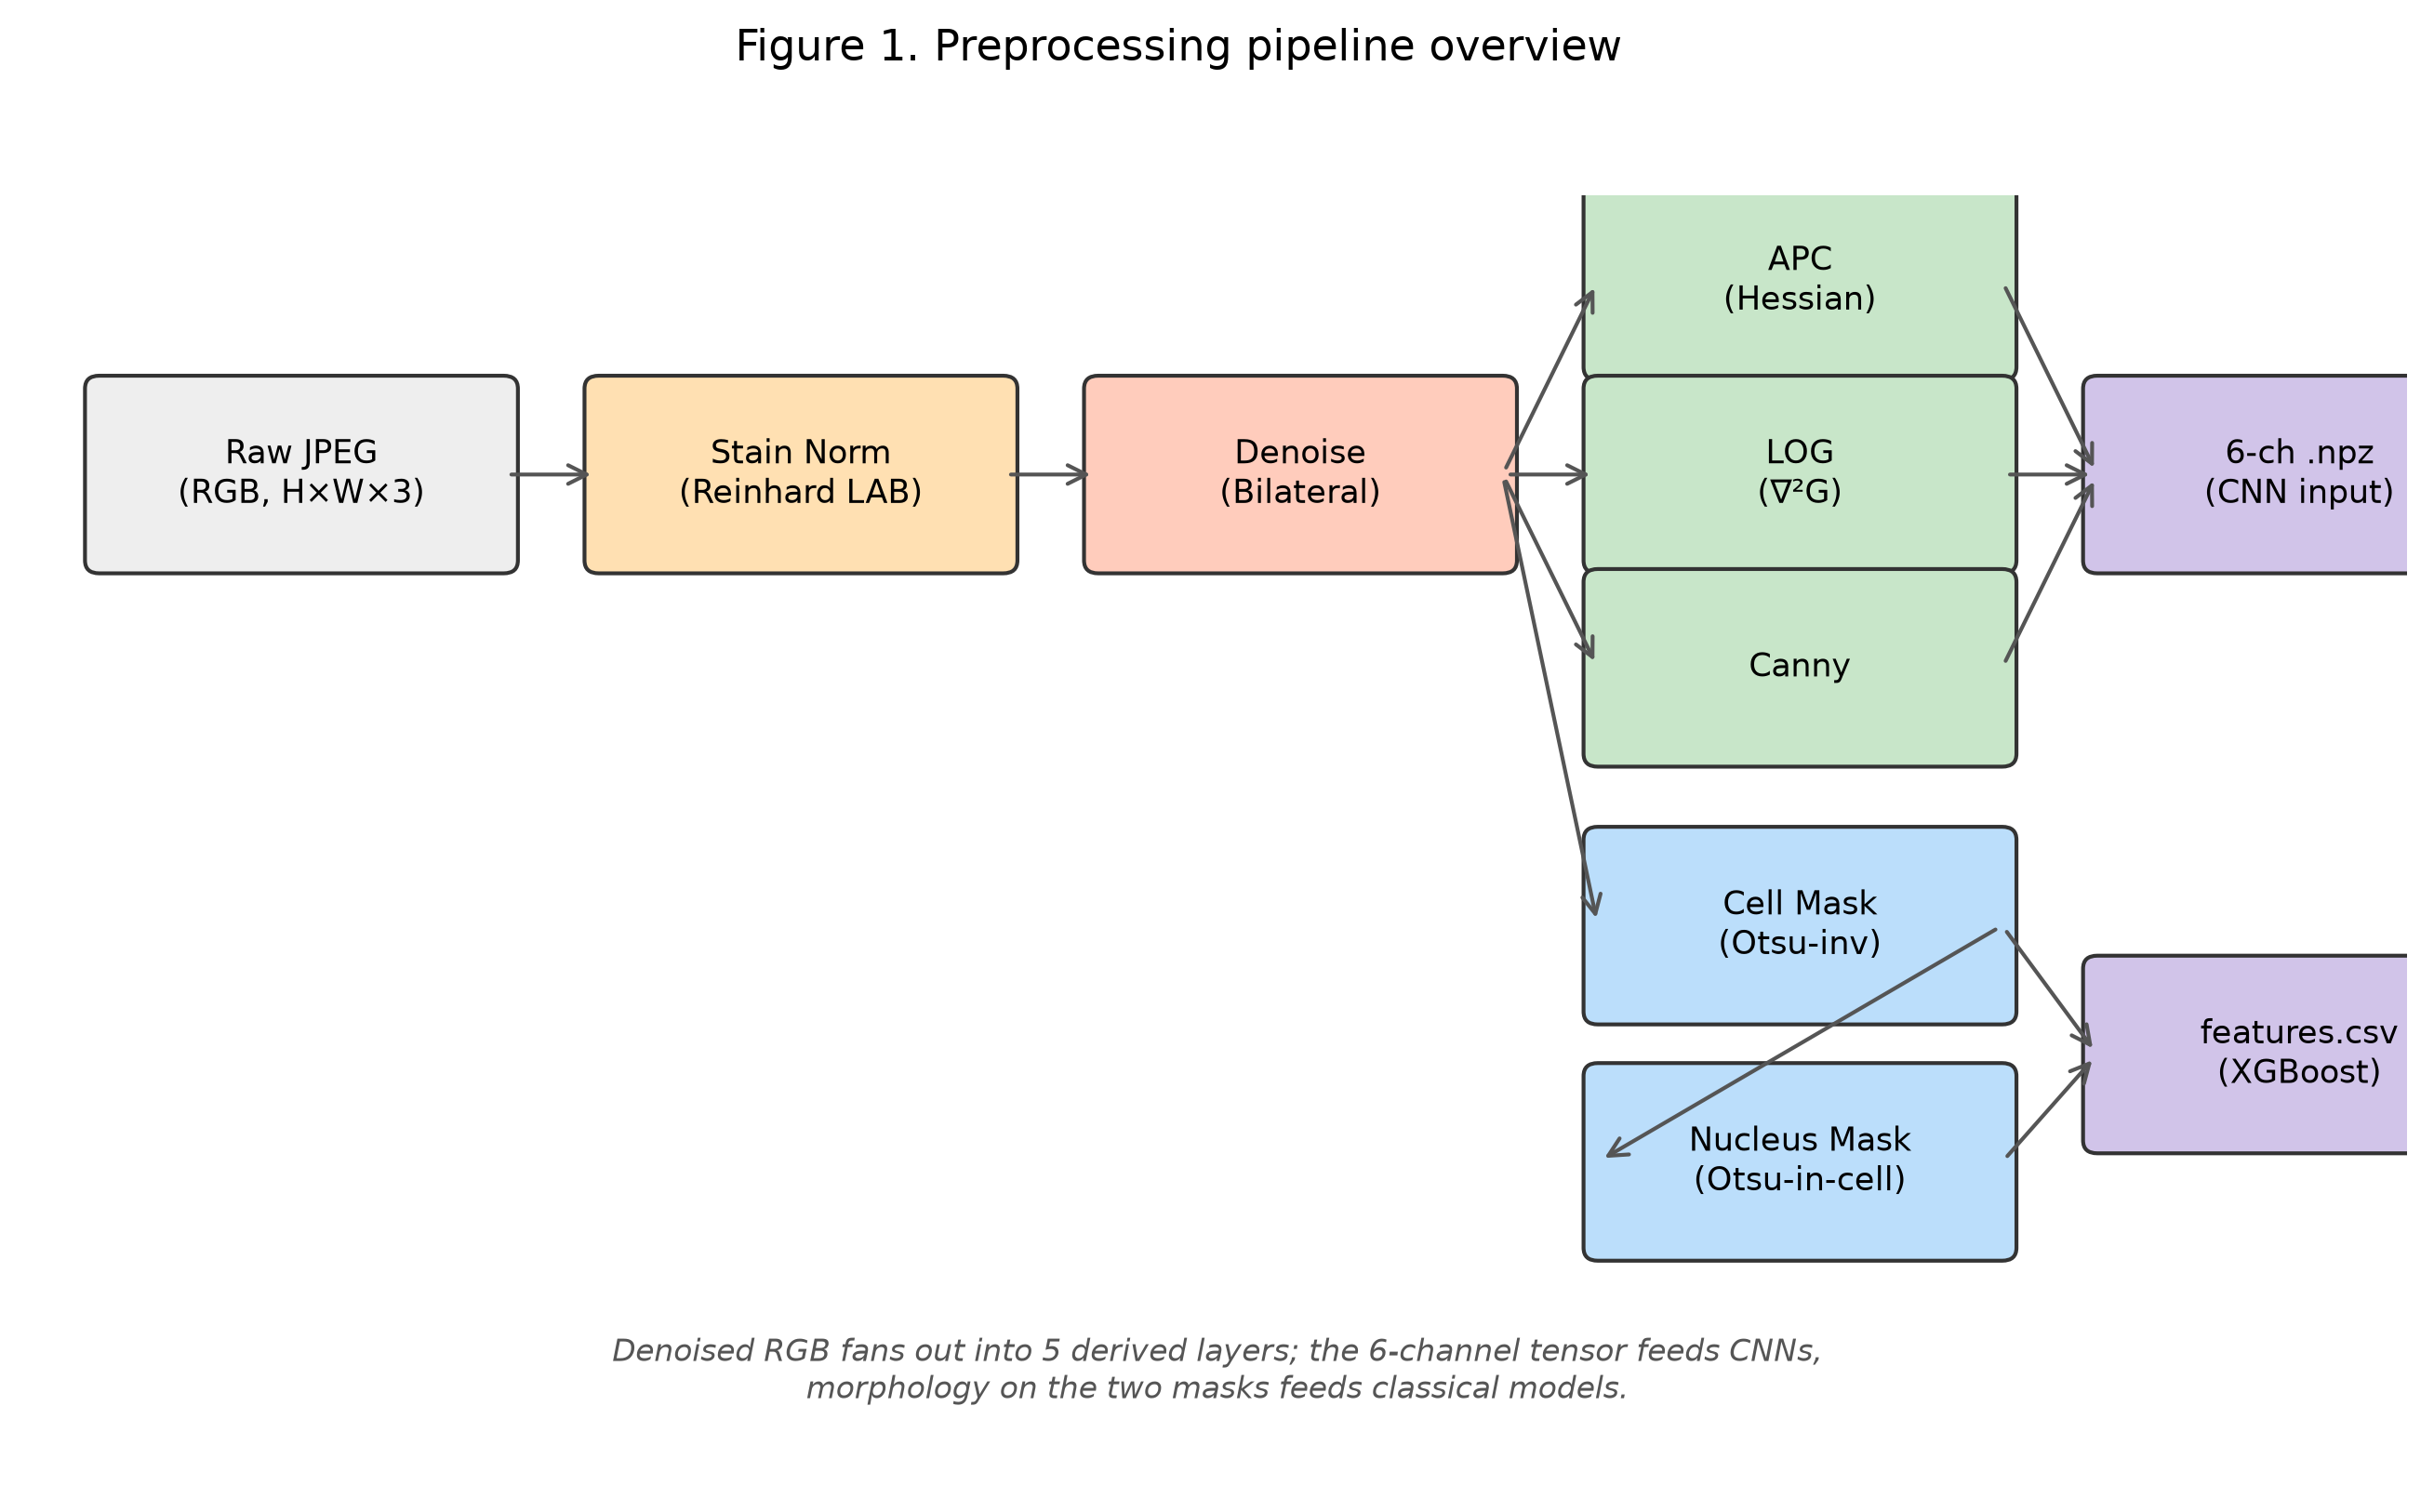
\includegraphics[width=\linewidth]{fig01_pipeline.png}
  \caption{Preprocessing pipeline overview. The raw JPEG passes through stain normalization and bilateral denoising, then fans out into five derived layers: three response maps (APC, LOG, Canny) feed a six-channel \texttt{.npz} tensor for convolutional models, while two binary masks (cell, nucleus) feed a morphological feature CSV for classical models.}
  \label{fig:pipeline}
\end{figure*}

% ==================================================================
\section{Background}
\label{sec:background}

We build on classical image-processing techniques rather than introducing new ones; the contribution is the composition and the rationale behind each choice.

\paragraph{Reinhard colour transfer.} Reinhard \emph{et~al.}~\cite{reinhard2001color} proposed matching the mean and standard deviation of a source image to a reference in perceptual $L^*a^*b^*$ space. Applied to H\&E micrographs, this operation removes scanner- and slide-specific colour drift while preserving intra-image contrast.

\paragraph{Bilateral filtering.} Tomasi and Manduchi~\cite{tomasi1998bilateral} introduced the bilateral filter, a Gaussian-weighted average whose weights are attenuated by intensity difference in addition to spatial distance. The filter smooths flat regions but preserves edges, which is precisely what the downstream Hessian and Laplacian operators require.

\paragraph{Hessian ridge detection.} Frangi \emph{et~al.}~\cite{frangi1998multiscale} used the eigenvalues of the image Hessian to detect tubular structures in retinal vessels. We use a simplified variant --- Adaptive Principal Curvature --- following the earlier Manvita blood-vessel work.

\paragraph{Laplacian of Gaussian.} Marr and Hildreth~\cite{marr1980theory} showed that the zero-crossings of $\nabla^2(G_\sigma * I)$ correspond to edges at scale $\sigma$; taking $|\nabla^2(G_\sigma * I)|$ yields a blob response tuned to structures of size $\approx \sigma\sqrt{2}$.

\paragraph{Canny edge detection.} Canny~\cite{canny1986computational} formalised the optimal single-scale edge detector via a chain of Gaussian smoothing, gradient computation, non-maximum suppression, and hysteresis thresholding.

\paragraph{Otsu thresholding.} Otsu~\cite{otsu1979threshold} selects the binary threshold that maximises inter-class variance, yielding a parameter-free segmentation baseline that we invert (cells stain darker than background) and further constrain (nuclei are the darkest region within cells).

\paragraph{GLCM texture.} Haralick~\cite{haralick1973textural} defined the gray-level co-occurrence matrix and derived fourteen texture descriptors from it; we use four (contrast, energy, homogeneity, correlation).

\paragraph{Perona--Malik and HDS.} Perona and Malik~\cite{perona1990scale} proposed a nonlinear diffusion PDE with an edge-stopping conduction coefficient. HDS extends this with a log-based prior term appropriate for \emph{multiplicative} speckle noise; we show in Section~\ref{sec:hds} that this term diverges on additive-Gaussian-noise microscopy data.

% ==================================================================
\section{Pipeline Overview}
\label{sec:overview}

Table~\ref{tab:stages} enumerates the seven stages in execution order. Each stage transforms an image (or set of images) and is implemented as a pure function to permit parallel execution via \texttt{multiprocessing.Pool}. We deliberately fit the stain reference from the training partition alone: any statistic derived from validation or test images would leak information into the model.

\begin{table*}[t]
  \centering
  \caption{The seven preprocessing stages, their inputs, outputs, and rationale.}
  \label{tab:stages}
  \begin{tabular}{@{}rlllp{5.5cm}@{}}
    \toprule
    \# & Stage                  & Input                & Output                            & Rationale \\
    \midrule
    1  & Stain Normalization    & Raw BGR              & Normalised BGR                    & Remove scanner/slide colour drift \\
    2  & Bilateral Denoising    & Normalised BGR       & Denoised BGR                      & Suppress sensor noise, preserve edges \\
    3  & APC Response           & Denoised grayscale   & $H \times W$ float                & Ridge/membrane detector, Hessian eigenvalues \\
    4  & LOG Response           & Denoised grayscale   & $H \times W$ float                & Blob detector, whole-cell scale \\
    5  & Canny Edges            & Denoised grayscale   & $H \times W$ boolean              & Sharp geometric edges \\
    6  & Cell Segmentation      & Denoised grayscale   & $H \times W$ boolean              & Inverted Otsu; cells stain dark \\
    7  & Nucleus Segmentation   & Denoised grayscale + cell mask & $H \times W$ boolean    & Otsu constrained to cell interior \\
    \bottomrule
  \end{tabular}
\end{table*}

% ==================================================================
\section{Stage-by-Stage Details}
\label{sec:stages}

\subsection{Stain Normalization (Reinhard)}
\label{sec:stain}

\paragraph{Purpose.} H\&E-stained microscopy images vary considerably in the hue and intensity of purple (haematoxylin) and pink (eosin) components. Reinhard normalization projects every image onto a common reference distribution in $L^*a^*b^*$ space, greatly reducing this nuisance variation.

\paragraph{Formulation.} Let $I(x)$ denote the source image in $L^*a^*b^*$ colour space with per-channel mean $\mu_{\mathrm{src}}$ and standard deviation $\sigma_{\mathrm{src}}$, and let $\mu_{\mathrm{ref}}, \sigma_{\mathrm{ref}}$ be the corresponding statistics of a reference distribution. The normalised image $I'(x)$ satisfies
\begin{equation}
  I'_c(x) = \frac{I_c(x) - \mu_{\mathrm{src},c}}{\sigma_{\mathrm{src},c}} \cdot \sigma_{\mathrm{ref},c} + \mu_{\mathrm{ref},c},
  \label{eq:reinhard}
\end{equation}
for each channel $c \in \{L^*, a^*, b^*\}$. The reference $(\mu_{\mathrm{ref}}, \sigma_{\mathrm{ref}})$ is obtained by averaging the per-image statistics across at most twenty training-partition Benign images:
\begin{equation}
  \mu_{\mathrm{ref}} = \frac{1}{N}\sum_{i=1}^{N} \mu_i, \qquad
  \sigma_{\mathrm{ref}} = \frac{1}{N}\sum_{i=1}^{N} \sigma_i.
\end{equation}
The clip $[0,255]$ is applied before converting back to BGR.

\paragraph{Leakage prevention.} Because $(\mu_{\mathrm{ref}}, \sigma_{\mathrm{ref}})$ are estimated once from training-partition data alone, no information about validation or test images propagates through the normalization step.

\paragraph{Empirical behaviour.} Figure~\ref{fig:stain} shows that on a well-stained image the transformation is a near-identity: source statistics already lie close to the reference distribution. On outlier slides (uncommon in the Aria dataset), the visible change is greater.

\begin{figure}[t]
  \centering
  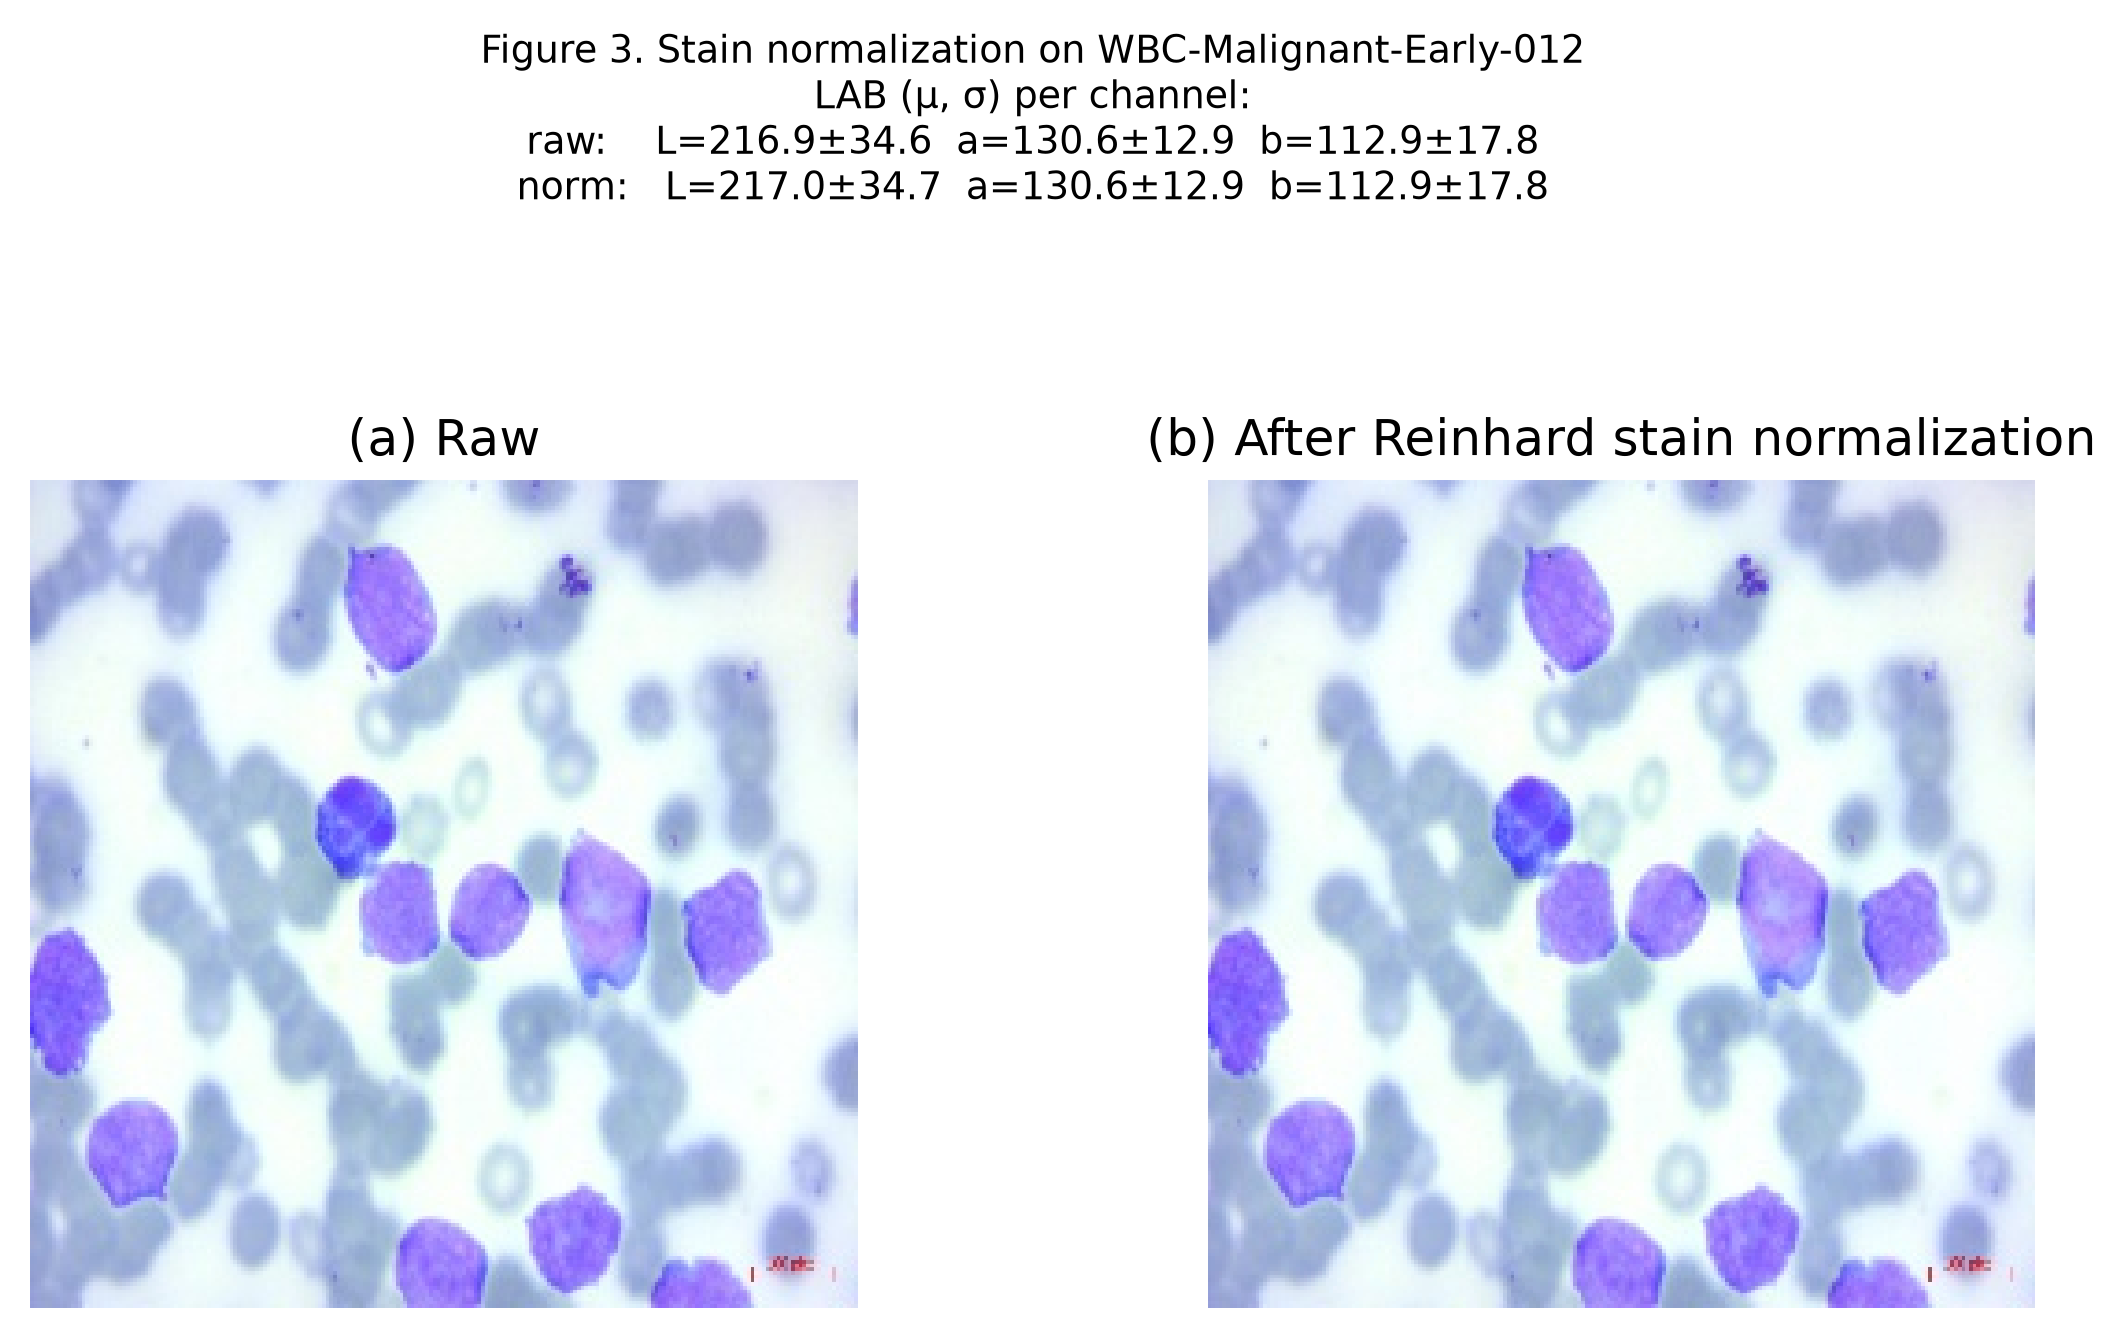
\includegraphics[width=\linewidth]{fig03_stain_norm.png}
  \caption{Reinhard stain normalization applied to WBC-Malignant-Early-012 with the image itself as the reference. The transformation is a near-identity; on outlier slides the effect is larger.}
  \label{fig:stain}
\end{figure}

% ------------------------------------------------------------------
\subsection{Denoising}
\label{sec:denoise}

\subsubsection{Bilateral Filter (chosen)}
\label{sec:bilateral}

\paragraph{Purpose.} Suppress sensor and JPEG-compression noise without blurring the cell membranes that downstream Hessian and Laplacian operators depend on.

\paragraph{Formulation.} The bilateral filter~\cite{tomasi1998bilateral} at pixel $x$ is
\begin{equation}
  I'(x) = \frac{1}{Z(x)} \sum_{y \in \mathcal{N}(x)}
          I(y)\, g_{\sigma_s}(\lVert x-y \rVert)\, g_{\sigma_r}(\lvert I(x)-I(y) \rvert),
  \label{eq:bilateral}
\end{equation}
where $g_\sigma$ is a Gaussian of standard deviation $\sigma$, $\mathcal{N}(x)$ is a $d \times d$ neighbourhood, $\sigma_s$ controls spatial smoothing and $\sigma_r$ controls tonal smoothing. $Z(x)$ is a normalising constant. We use OpenCV's implementation with $d=9$, $\sigma_s = \sigma_r = 75$.

\paragraph{Effect.} Figure~\ref{fig:bilateral} illustrates the effect on a 60-pixel crop of Early-012: the filter suppresses fine background noise while preserving the sharp boundary of the nearby cell.

\begin{figure}[t]
  \centering
  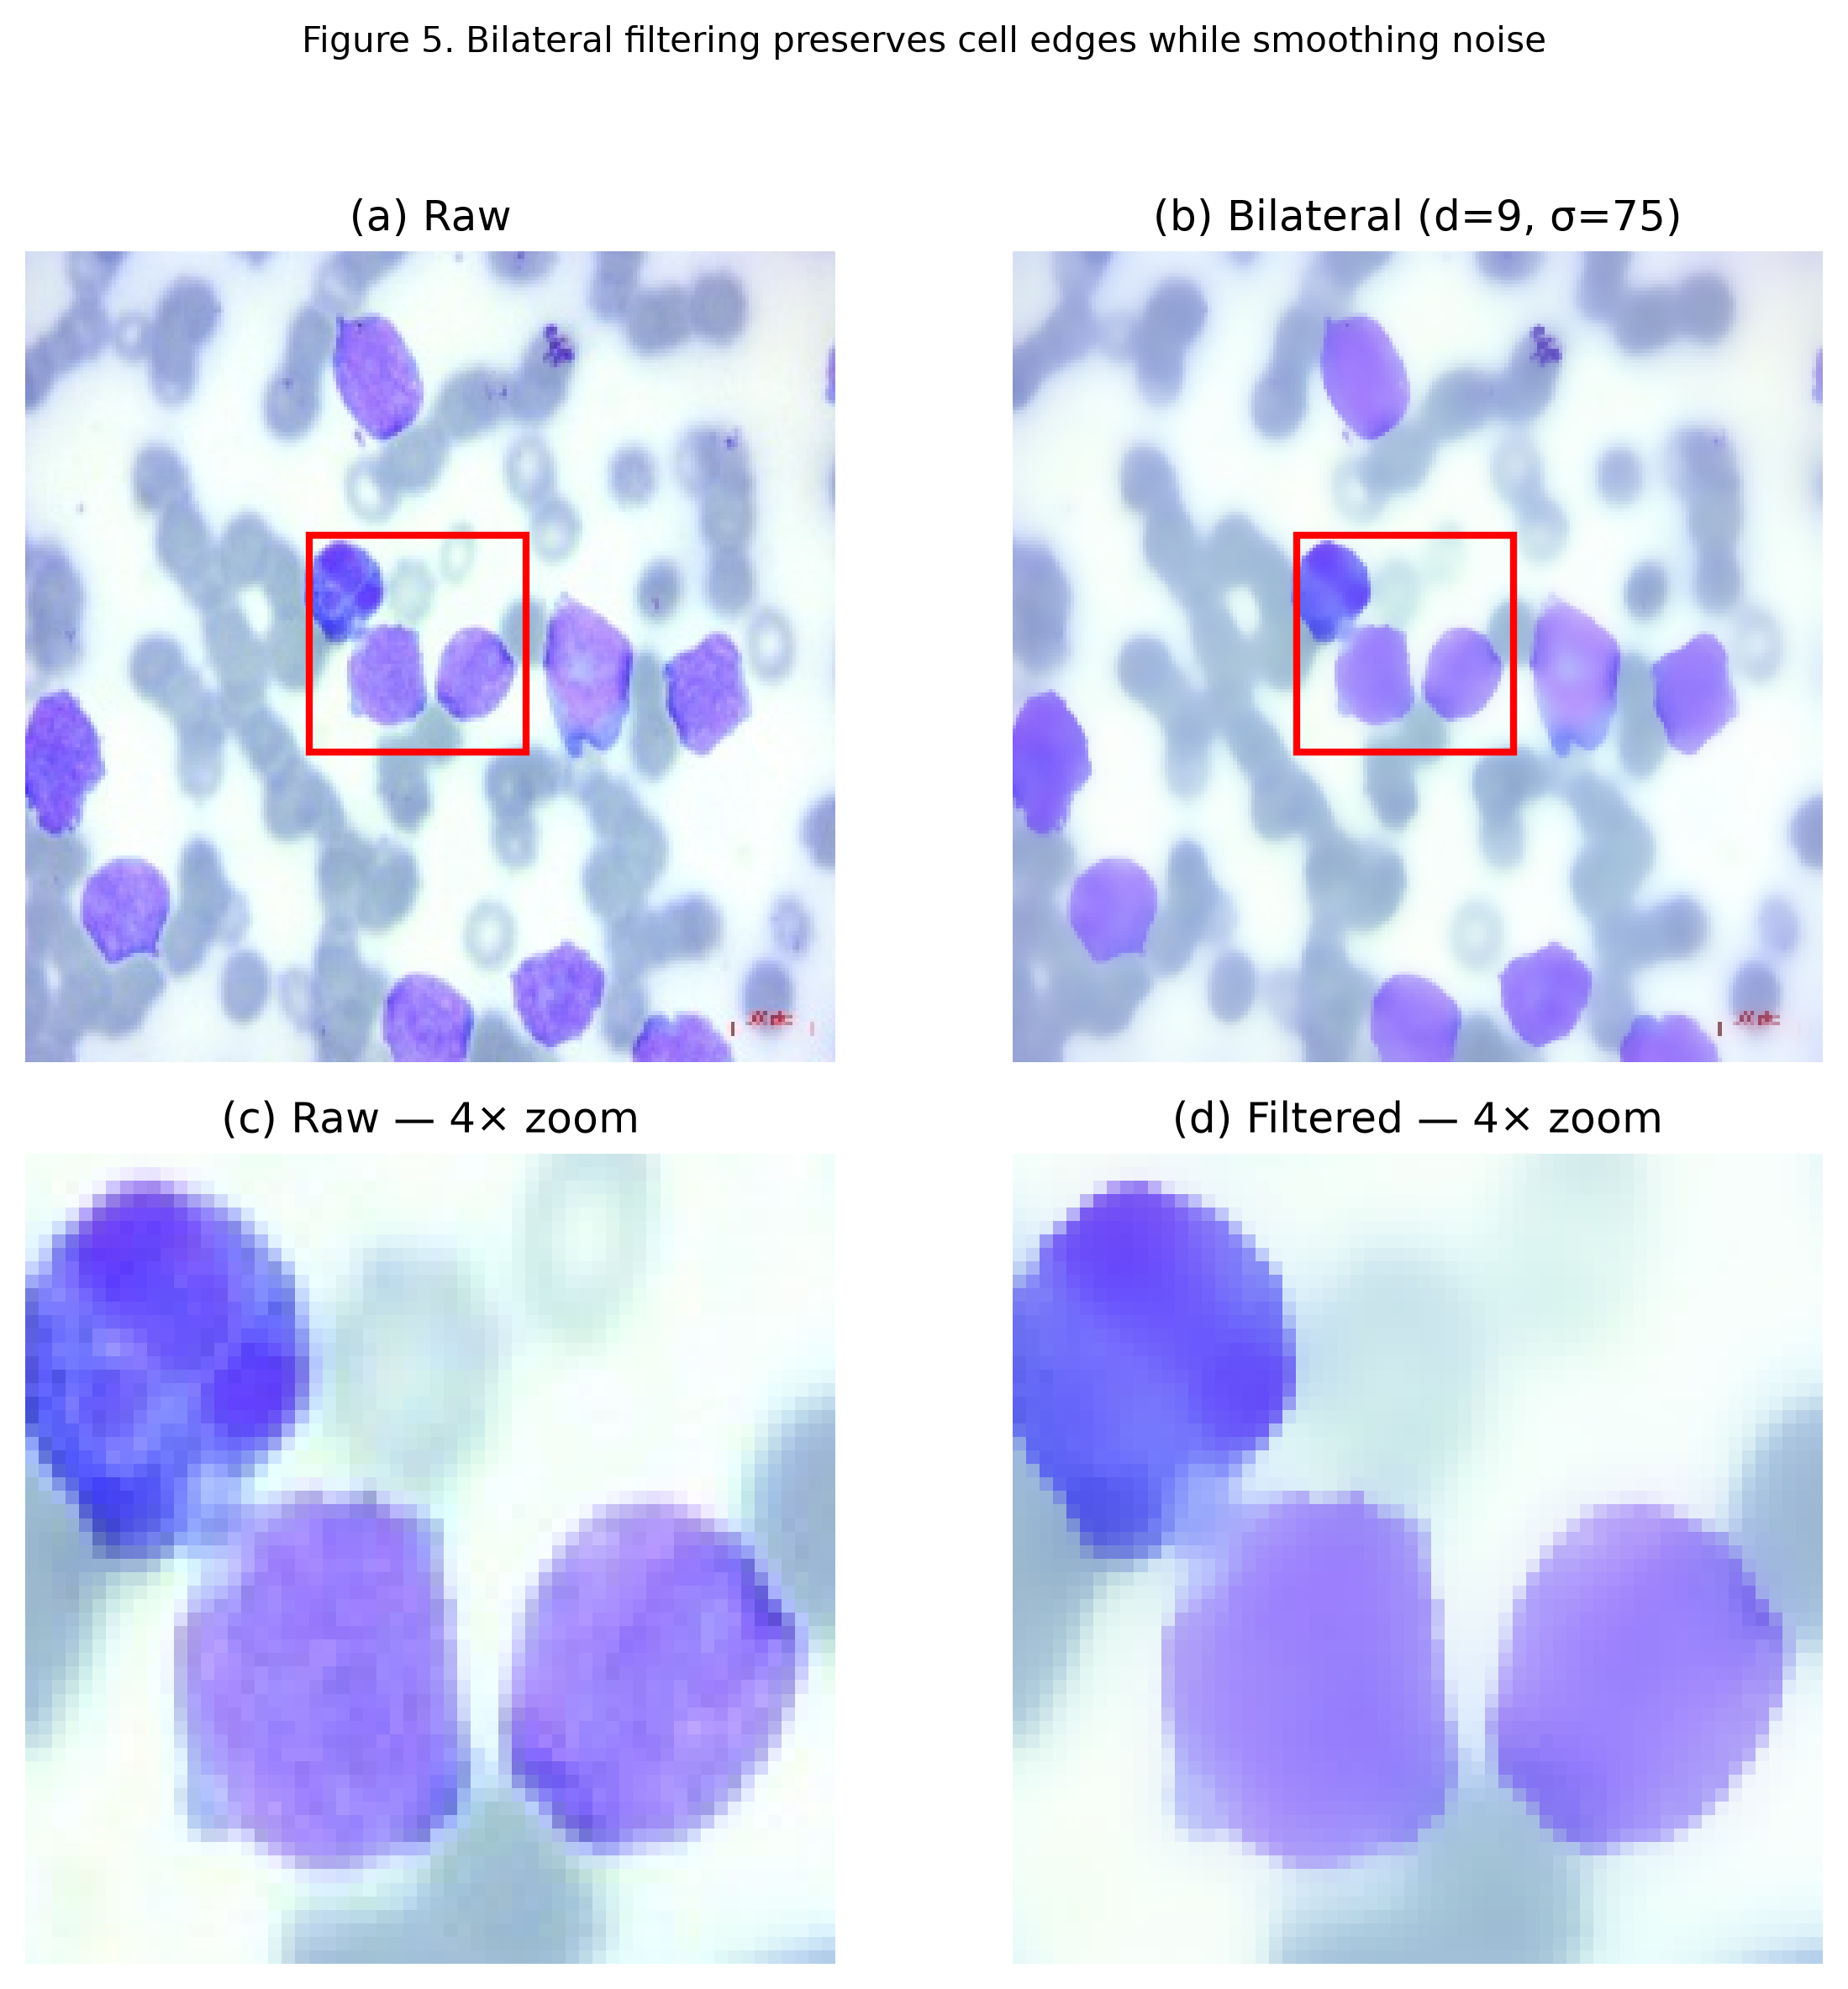
\includegraphics[width=\linewidth]{fig05_bilateral_zoom.png}
  \caption{Bilateral filtering with a 60-pixel zoomed inset. Cell edges remain sharp; flat regions are smoothed.}
  \label{fig:bilateral}
\end{figure}

\subsubsection{HDS (rejected): a Cautionary Analysis}
\label{sec:hds}

We initially considered the Hybrid Diffusion-Steered (HDS) denoiser inherited from Block~2 of the wider Manvita project. HDS combines Perona--Malik anisotropic diffusion with a log-prior term appropriate for multiplicative speckle noise. Its steepest-descent update for a scalar image $u$ with original observation $f$ is
\begin{equation}
  u^{(n+1)} = u^{(n)} + \Delta t \left[ D(u^{(n)}) - P(u^{(n)}, f) \right],
  \label{eq:hds}
\end{equation}
where the diffusion term is
\begin{equation}
  D(u) = \sum_{k \in \{N,S,W,E\}} c_k(u)\, \nabla_k u,
\end{equation}
with edge-stopping coefficients
\begin{equation}
  c_k(u) = G \left( \frac{1}{1 + (\nabla_k u)^2 / H^2}
                  + \frac{1}{|\nabla_k u| + \epsilon} \right),
\end{equation}
and the log-based fidelity term is
\begin{equation}
  P(u, f) = \lambda \left(\frac{u}{f + \epsilon} - 1\right) \frac{1}{u + \epsilon}.
  \label{eq:logprior}
\end{equation}

\paragraph{The divergence.} Equation~(\ref{eq:logprior}) is well-behaved when $u$ and $f$ stay in the interior of $(0,1)$. Trouble arises for dark pixels: as $u \to 0^+$, the factor $1/(u+\epsilon)$ diverges while the sign of $(u/f - 1)$ is negative (since $u < f$ typically holds early in iteration). Consequently $-P$ (the term actually applied to $u$) becomes strongly \emph{positive}: dark pixels are driven brighter with unbounded rate. Simultaneously, bright pixels see $u/f \approx 1$ and $P \approx 0$, so they drift slowly. Over hundreds of iterations the image converges to a bimodal equilibrium in which the majority of pixels are pinned at either $0$ or $1$ after clipping, and the three colour channels' means collapse to indistinguishable values.

\paragraph{Empirical confirmation.} Figure~\ref{fig:hds} shows this collapse quantitatively. On WBC-Malignant-Early-012:
\begin{itemize}
  \item Raw:   $\mu = 218$, $\sigma = 40$ (structured pinkish distribution).
  \item Bilateral: $\mu = 218$, $\sigma = 39$ (near-identity on mean/std but smoothed spatially).
  \item HDS, 20 iterations:  $\mu = 164$, $\sigma = 104$.
  \item HDS, 200 iterations: $\mu = 160$, $\sigma = 106$.
\end{itemize}
Note that all three colour channels of the HDS output converge to the same mean, which is the visual signature of the equilibrium described above.

\begin{figure*}[t]
  \centering
  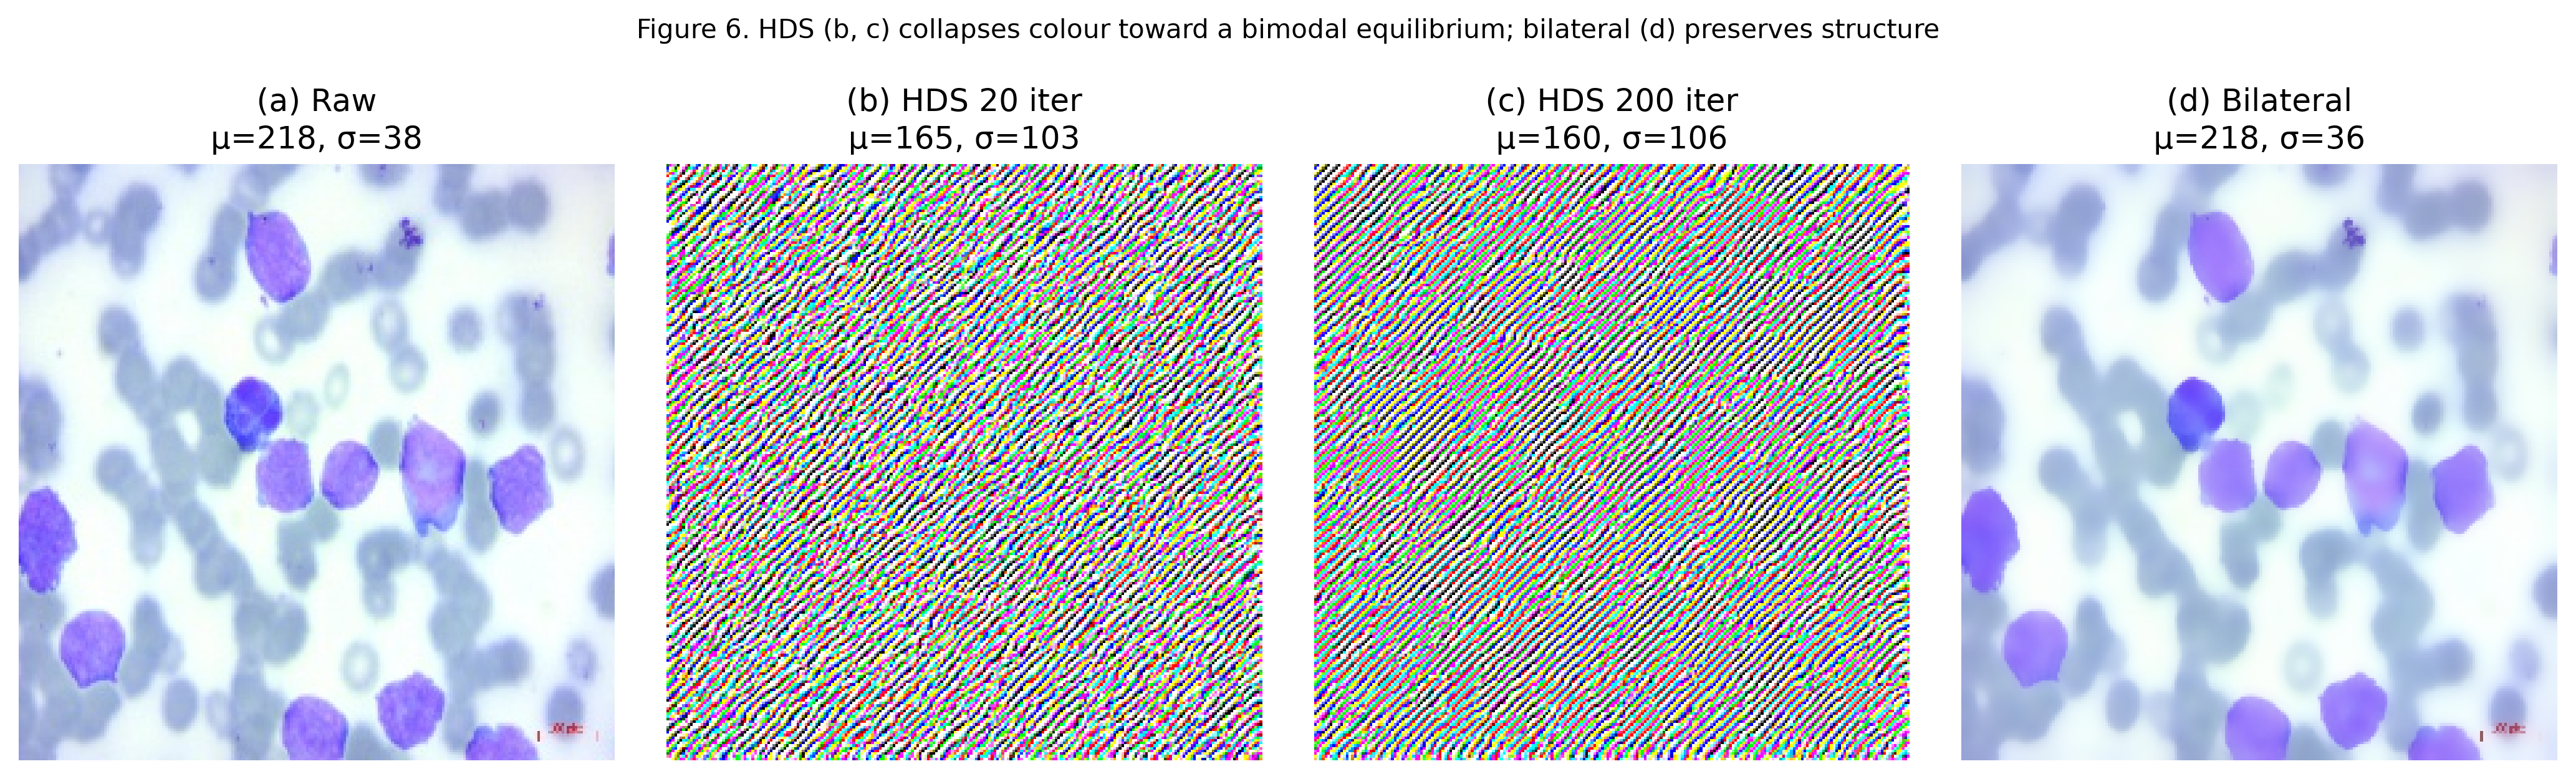
\includegraphics[width=\linewidth]{fig06_hds_divergence.png}
  \caption{The HDS denoiser diverges to a bimodal equilibrium on natural microscopy. After only 20 iterations the RGB channels have collapsed to identical means with $\sigma \approx 104$; the 200-iteration result is qualitatively identical.
  Bilateral filtering (rightmost panel) preserves both structure and colour.}
  \label{fig:hds}
\end{figure*}

\paragraph{Lesson.} HDS is not a general-purpose denoiser; it is a maximum-a-posteriori estimator under a specific noise model (multiplicative speckle, as encountered in SAR or ultrasound imaging). Applying it to additive-Gaussian-noise natural imagery drives the equations outside their region of validity. We retain the HDS implementation in \texttt{core.py} behind a \texttt{DENOISE\_METHOD} configuration switch for methodological comparisons but do not use it in the production pipeline.

% ------------------------------------------------------------------
\subsection{Adaptive Principal Curvature (APC)}
\label{sec:apc}

\paragraph{Purpose.} Detect ridge-like structures whose scale approximates that of a WBC nuclear membrane.

\paragraph{Formulation.} Let $I_\sigma = G_\sigma * I$ denote the Gaussian-smoothed image at scale $\sigma$. The Hessian matrix of second-order partial derivatives at pixel $x$ is
\begin{equation}
  H(x) = \begin{pmatrix} I_{xx}(x) & I_{xy}(x) \\ I_{xy}(x) & I_{yy}(x) \end{pmatrix}.
\end{equation}
Its eigenvalues $\lambda_1(x), \lambda_2(x)$ with $|\lambda_1| \le |\lambda_2|$ are the principal curvatures; a ridge is characterised by $|\lambda_2| \gg |\lambda_1|$. The APC response combines the two curvatures linearly:
\begin{equation}
  \mathrm{APC}(x) = \alpha |\lambda_2(x)| + (1 - \alpha) |\lambda_1(x)|,
  \label{eq:apc}
\end{equation}
followed by min--max normalisation to $[0, 1]$. We choose $\sigma = 2.5$ and $\alpha = 0.6$ to bias the detector toward the dominant curvature direction while retaining sensitivity to two-directional structures such as nucleoli.

\paragraph{Scale choice.} A nuclear membrane is typically 5--15 pixels thick in the Aria dataset; $\sigma = 2.5$ tunes the second-derivative operator to the correct receptive field. Smaller $\sigma$ produces a sub-pixel edge map dominated by JPEG artifacts; larger $\sigma$ merges adjacent cells.

\paragraph{Result.} Figure~\ref{fig:apc} shows the APC map on all three demonstration images: every cell (both WBCs and erythrocytes) is traced by a bright ring precisely at its membrane.

\begin{figure}[t]
  \centering
  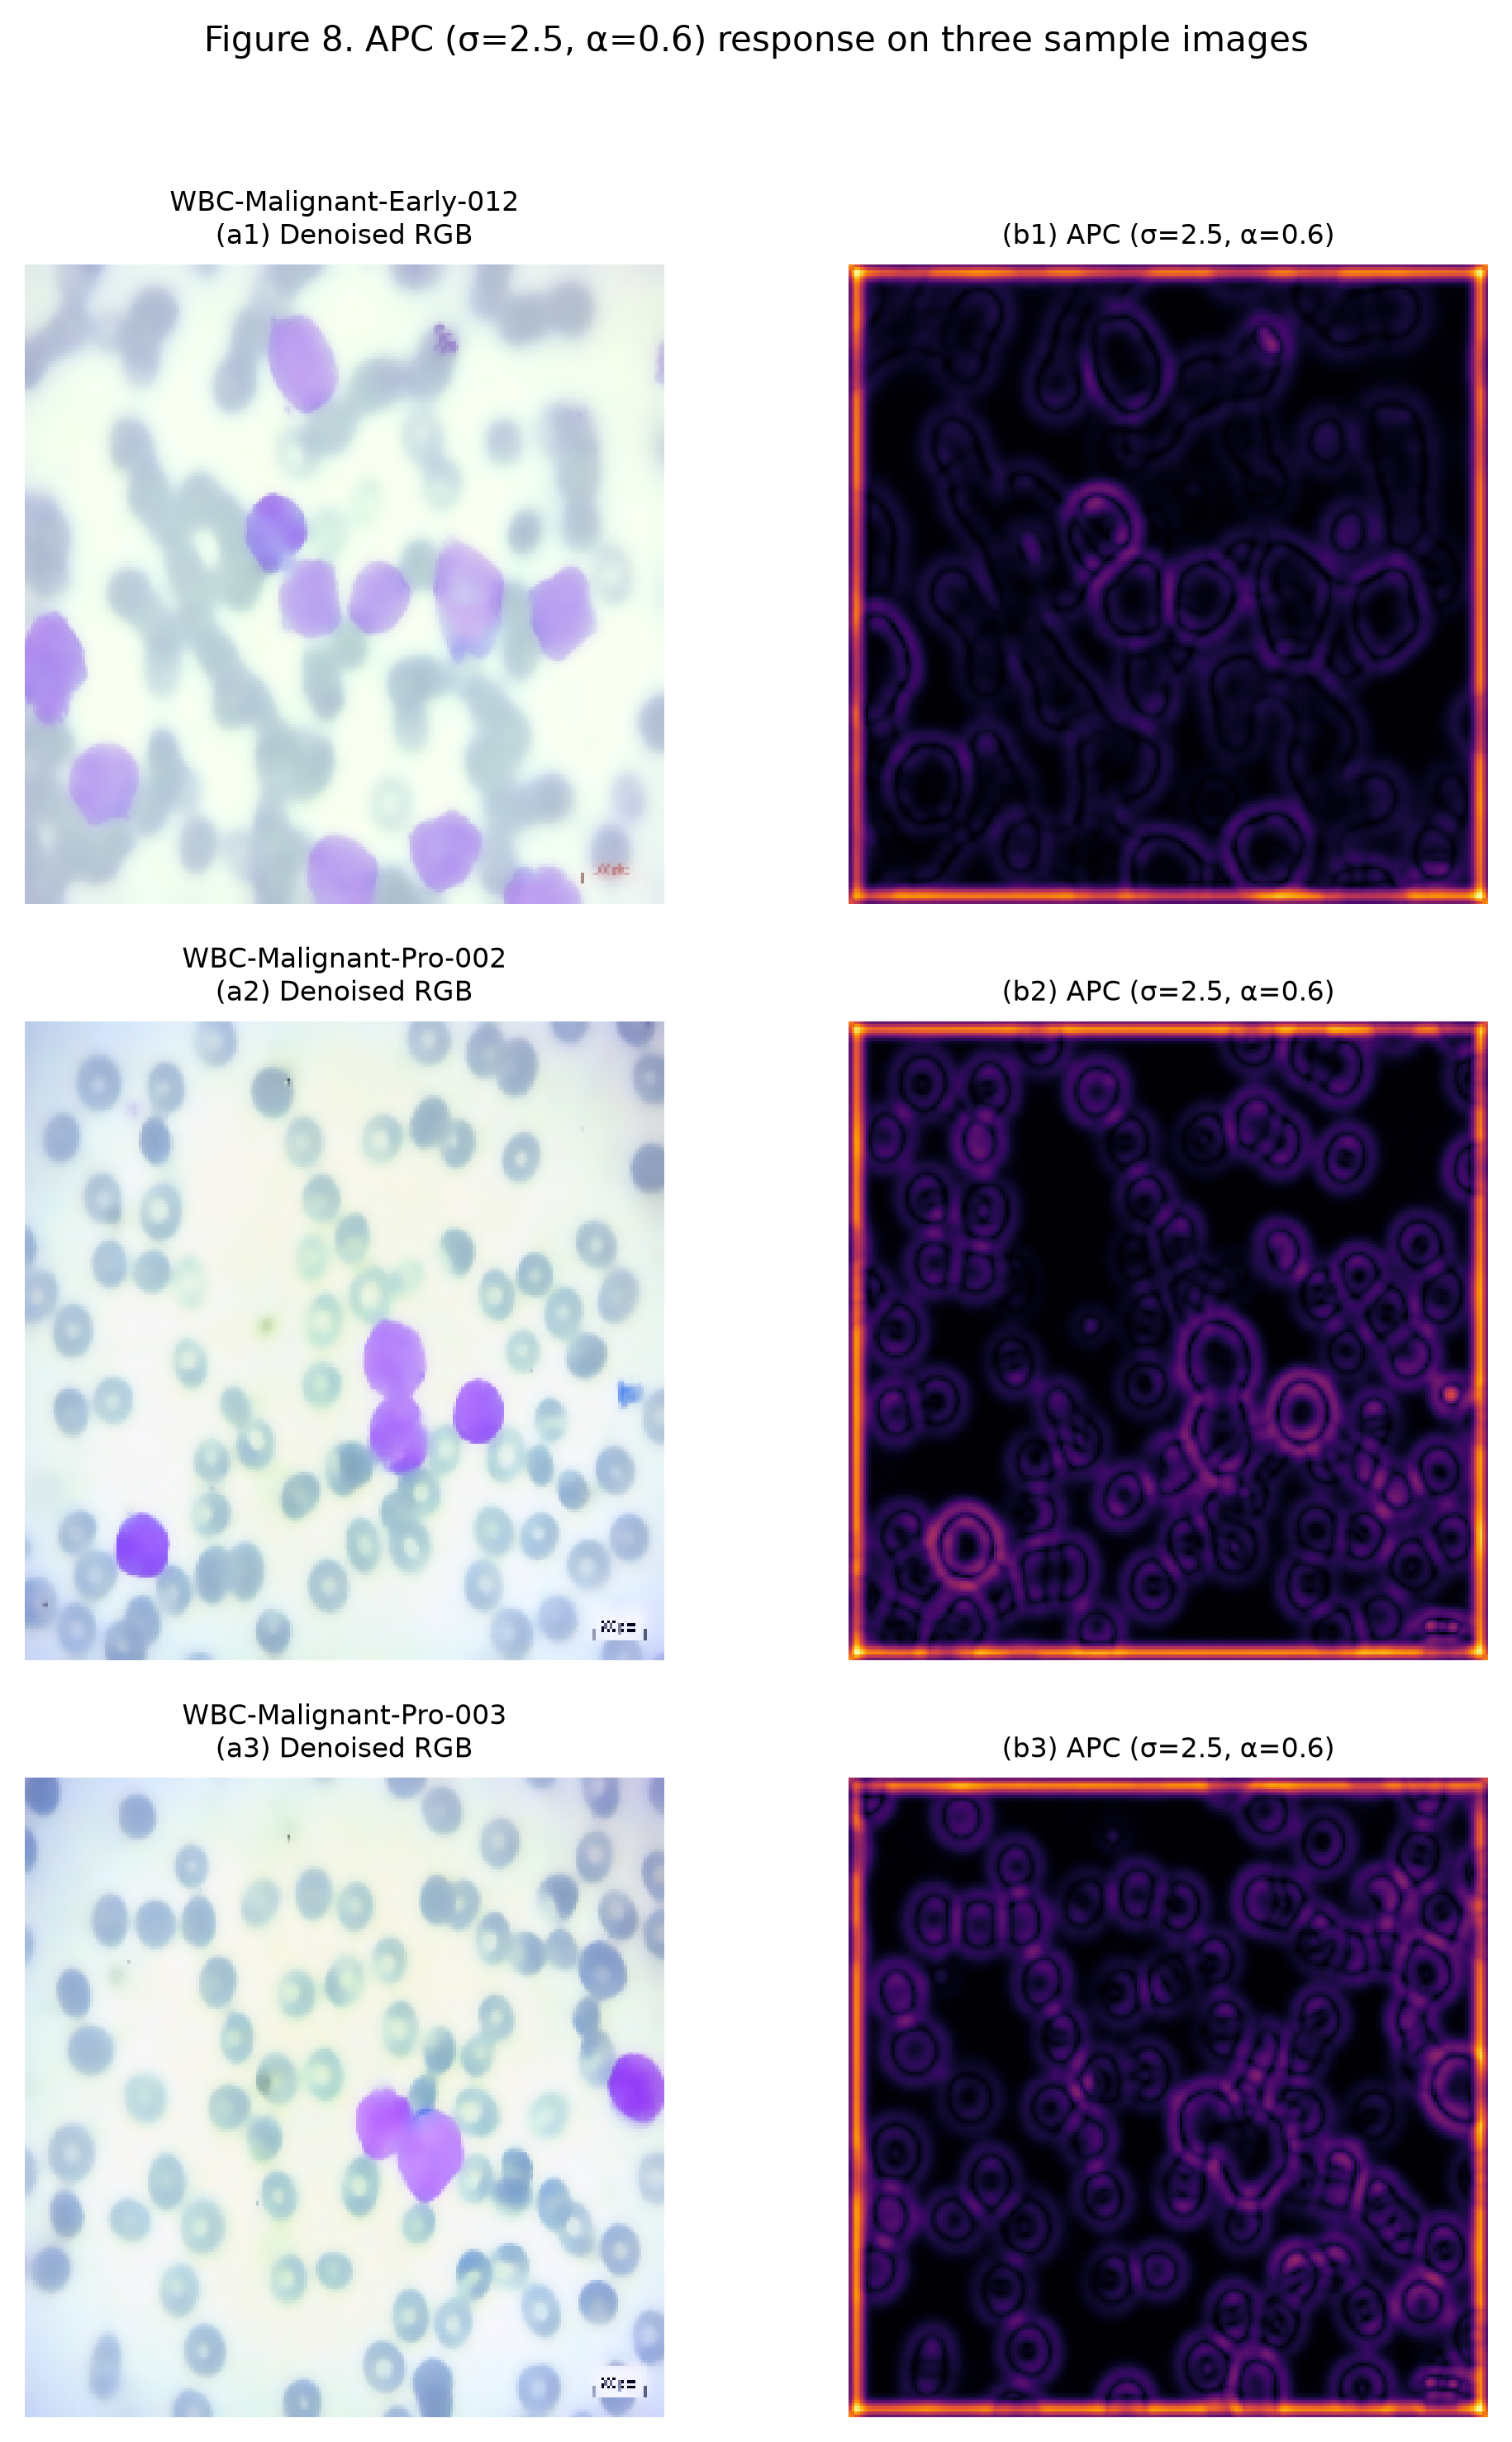
\includegraphics[width=\linewidth]{fig08_apc.png}
  \caption{APC response (right column) on the three demo images. Every cell rim is traced by a bright ring; nucleoli in the WBCs also appear.}
  \label{fig:apc}
\end{figure}

% ------------------------------------------------------------------
\subsection{Laplacian of Gaussian (LOG)}
\label{sec:log}

\paragraph{Purpose.} Detect blob-like structures at the scale of a whole cell.

\paragraph{Formulation.} The LOG response at scale $\sigma$ is
\begin{equation}
  \mathrm{LOG}_\sigma(x) = \left| \nabla^2 (G_\sigma * I)(x) \right|,
  \label{eq:log}
\end{equation}
followed by min--max normalisation. We use $\sigma = 4.0$, roughly matching the radius of a mature erythrocyte in these images.

\paragraph{Result.} Figure~\ref{fig:log} shows that the LOG response places its highest values at the interiors of cells rather than at their edges (in contrast to APC), making it complementary as a CNN input channel: APC contributes rim information, LOG contributes centroid information.

\begin{figure}[t]
  \centering
  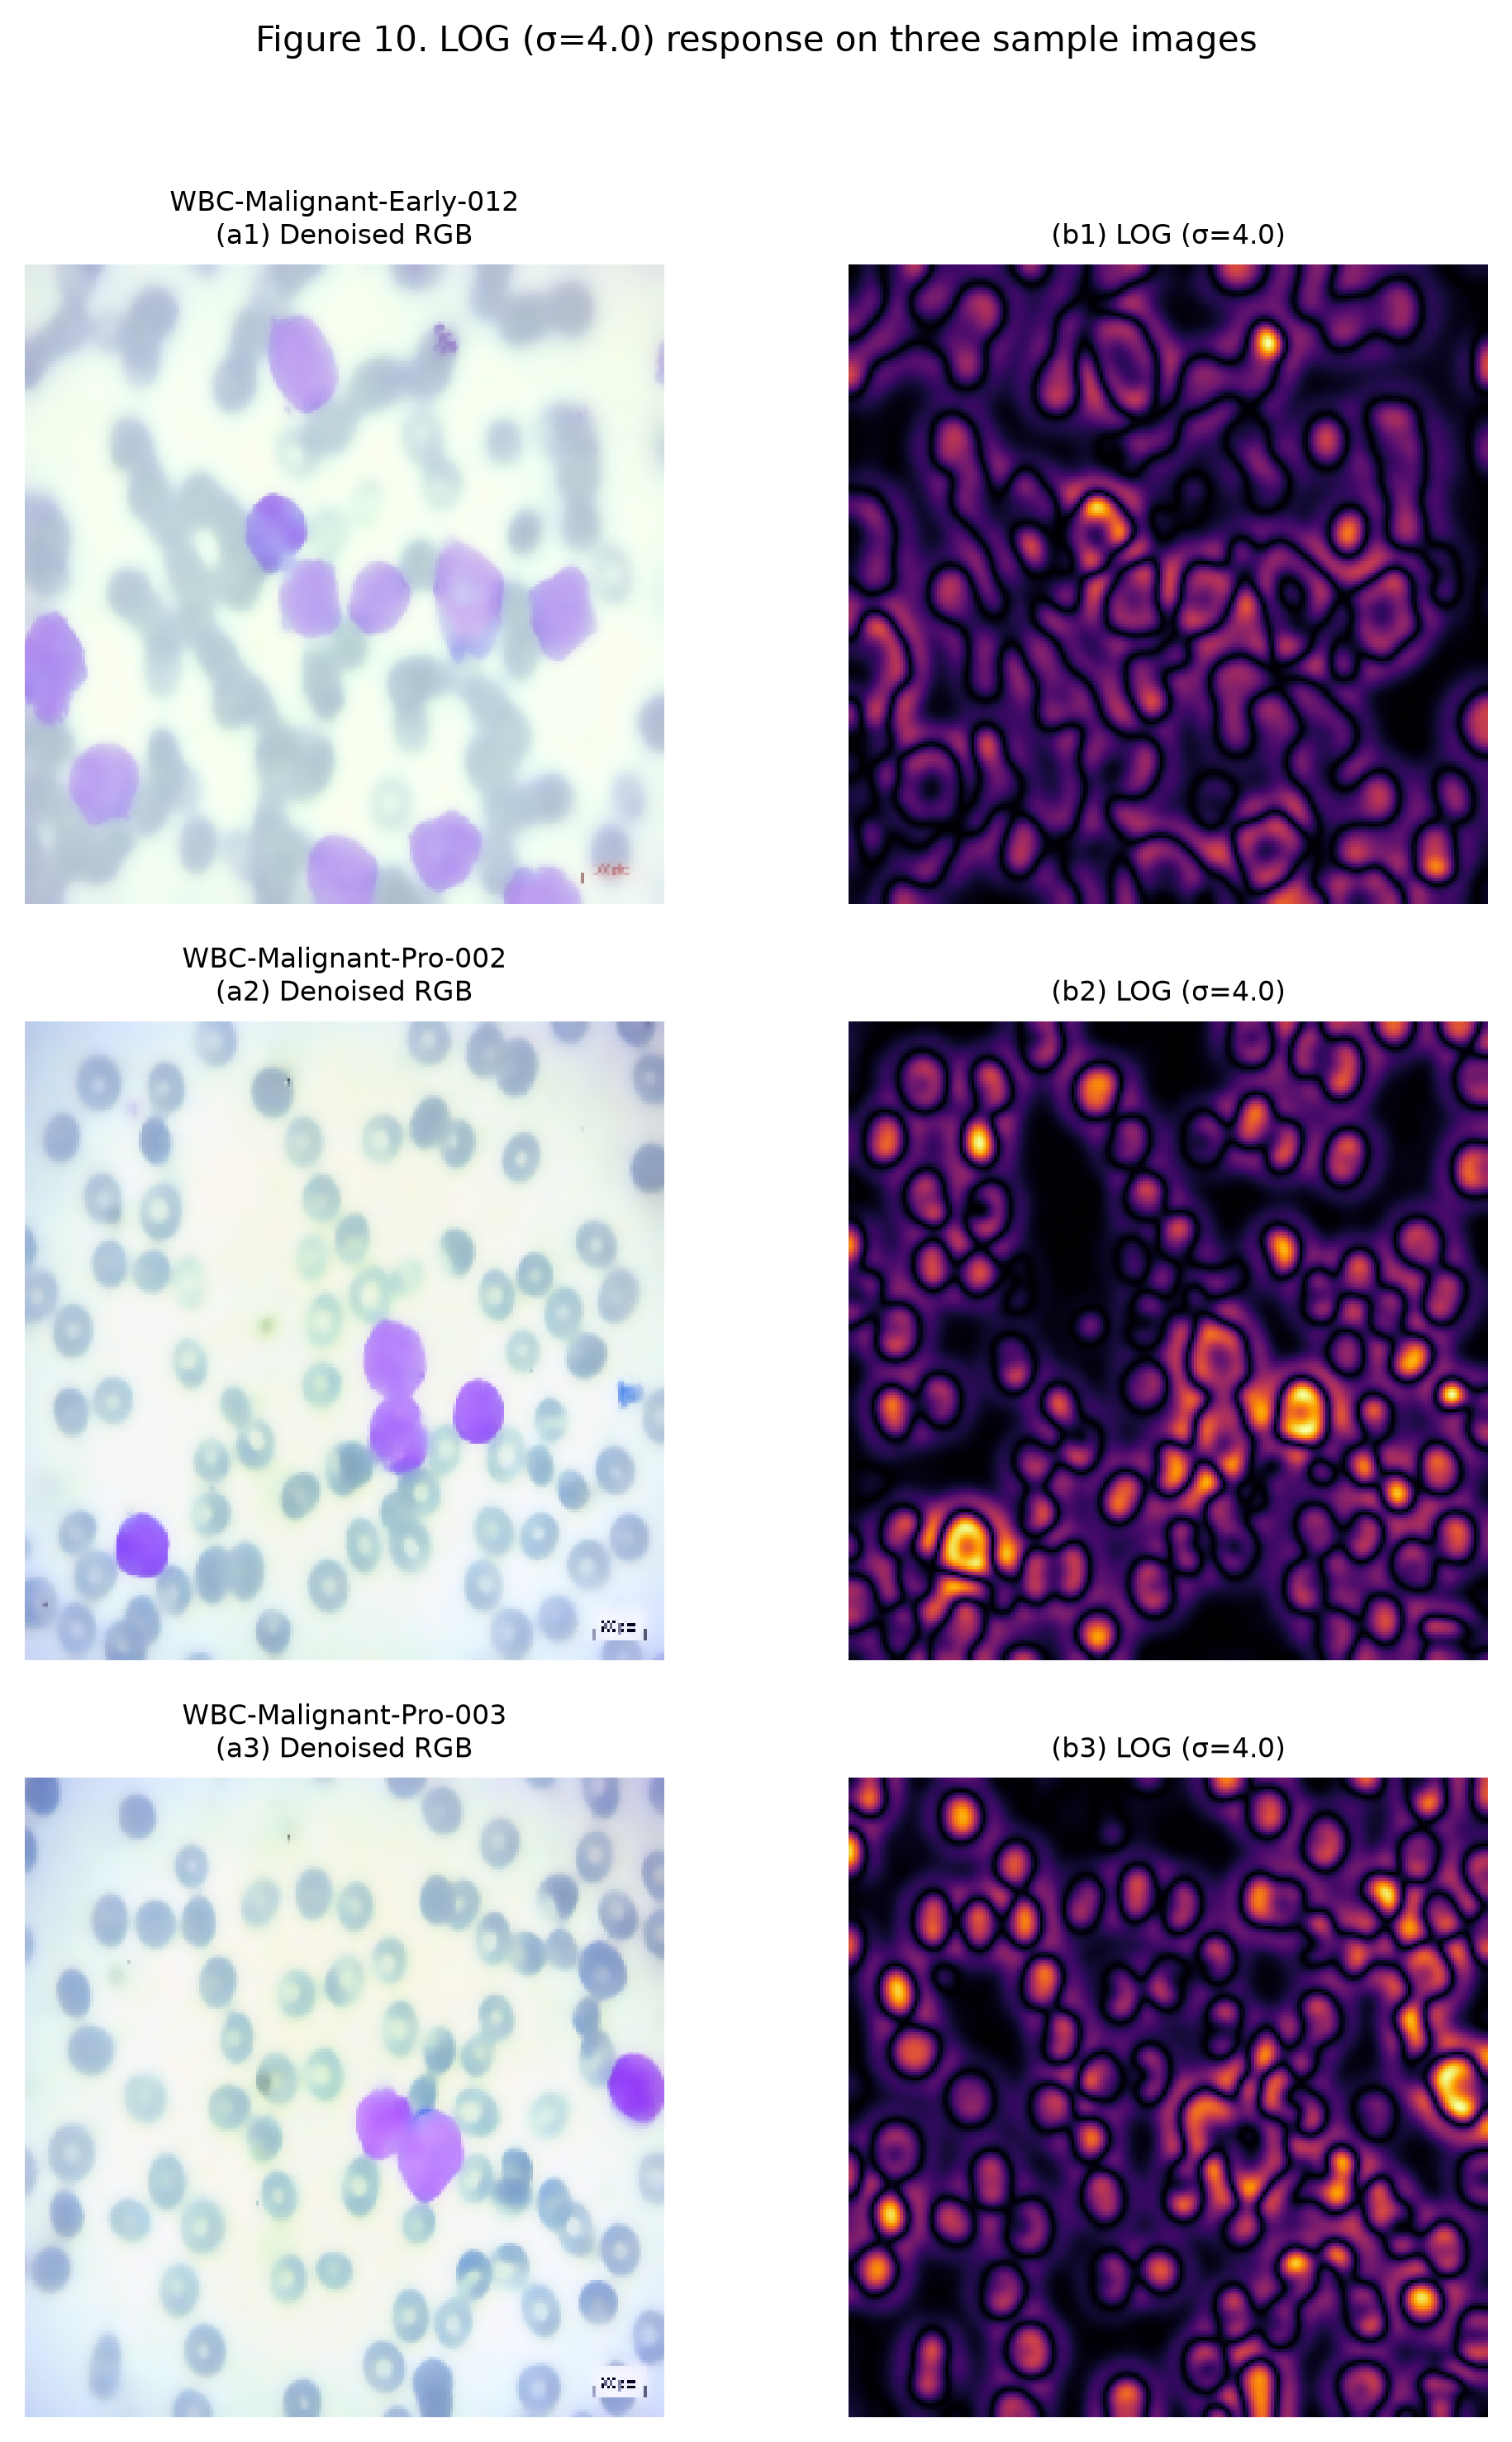
\includegraphics[width=\linewidth]{fig10_log.png}
  \caption{LOG response with $\sigma = 4.0$. Bright hotspots mark cell centres; darker halos surround them.}
  \label{fig:log}
\end{figure}

% ------------------------------------------------------------------
\subsection{Canny Edge Detection}
\label{sec:canny}

\paragraph{Purpose.} A crisp binary edge map complementary to the graded APC and LOG responses.

\paragraph{Formulation.} The Canny detector~\cite{canny1986computational} proceeds in four steps: (i) Gaussian smoothing at scale $\sigma$; (ii) gradient magnitude and orientation via Sobel; (iii) non-maximum suppression along the gradient direction; (iv) hysteresis thresholding with a low threshold $\tau_l$ and a high threshold $\tau_h$. A pixel is retained if its gradient magnitude exceeds $\tau_h$ or if it exceeds $\tau_l$ and is connected via a chain of $\ge \tau_l$ pixels to a $\ge \tau_h$ pixel.

We use OpenCV's implementation with $\tau_l = 0.1$ and $\tau_h = 0.25$ (both in units of normalised intensity), applied to the bilateral-denoised grayscale image.

\paragraph{Result.} Figure~\ref{fig:canny} shows continuous closed contours around every cell.

\begin{figure}[t]
  \centering
  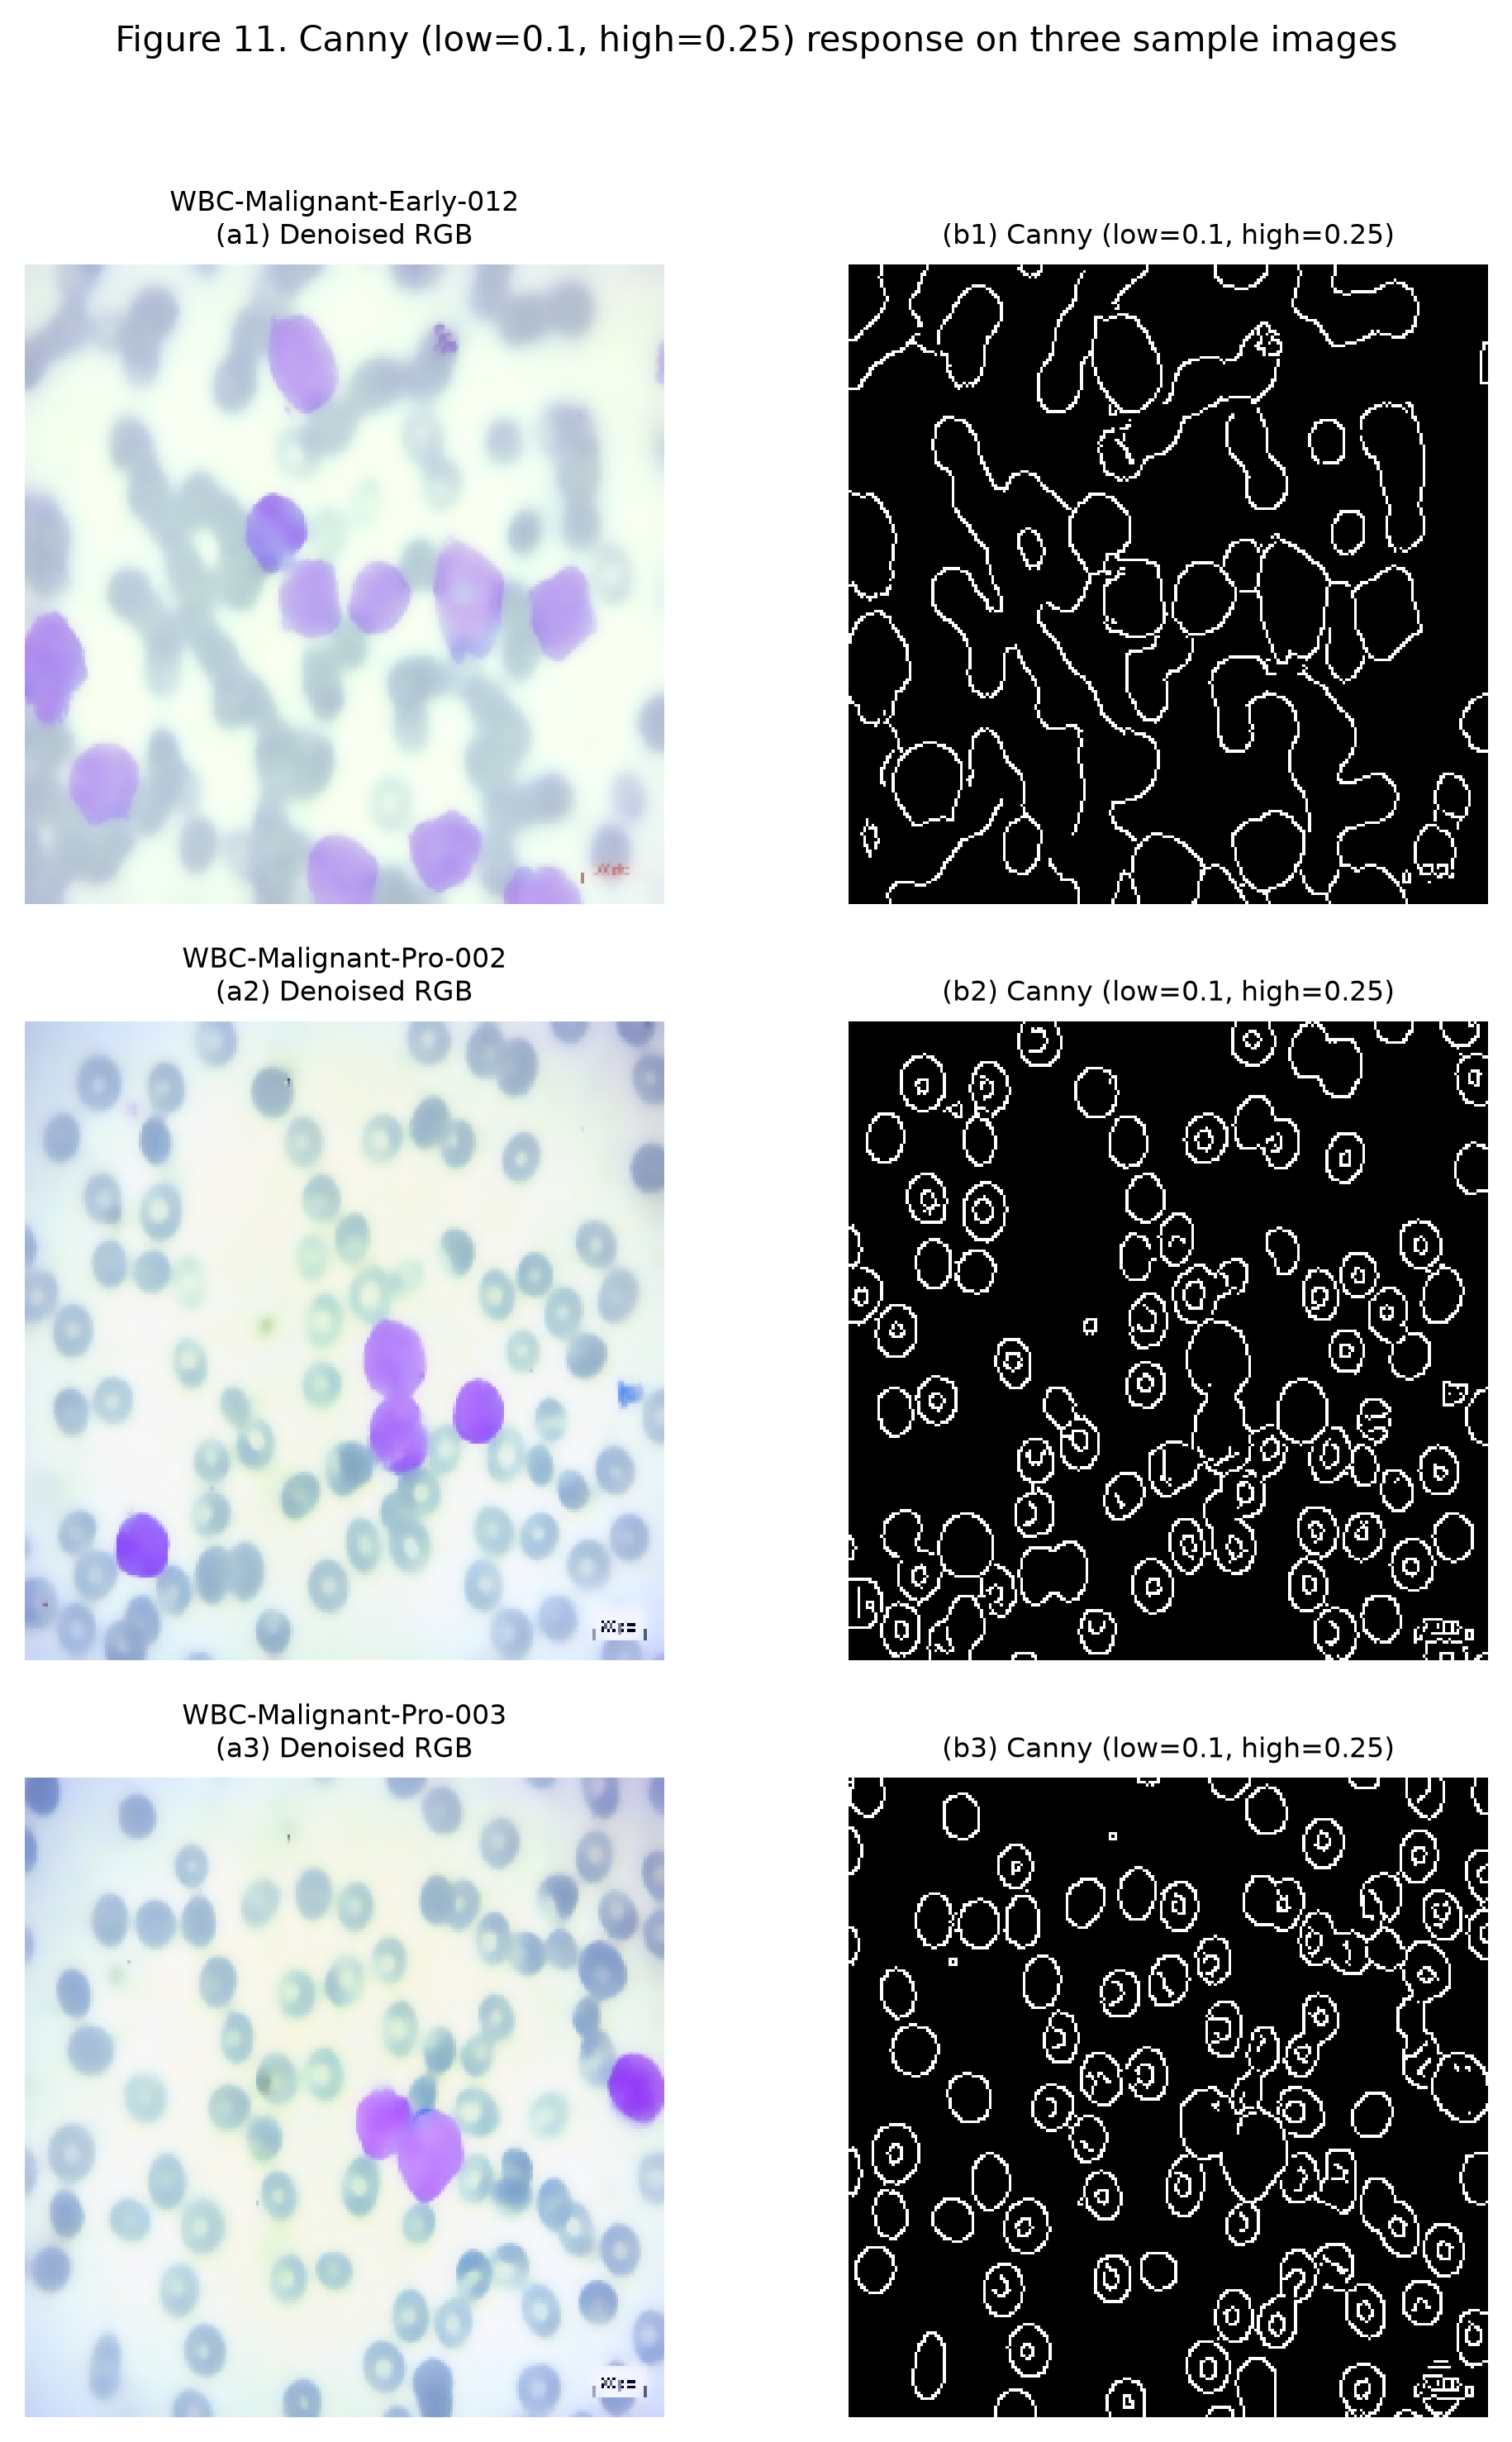
\includegraphics[width=\linewidth]{fig11_canny.png}
  \caption{Canny binary edges at $\tau_l = 0.1$, $\tau_h = 0.25$.}
  \label{fig:canny}
\end{figure}

% ------------------------------------------------------------------
\subsection{Cell Segmentation (inverted Otsu)}
\label{sec:cellseg}

\paragraph{Purpose.} Produce a binary mask of all cell bodies for use as a segmentation prior and as the domain over which nucleus segmentation is subsequently performed.

\paragraph{Method.} Cells stain darker than background in Wright/Giemsa preparations. Let $g(x)$ denote the denoised grayscale intensity of a pixel. We select Otsu's optimum threshold $\tau^*$ and construct
\begin{equation}
  M_{\mathrm{cell}}(x) = \mathbb{1}[g(x) < \tau^*].
\end{equation}
Morphological closing with a disk of radius $r_c = 5$ fills small intra-cell gaps, and a size filter removes components smaller than $100$ pixels.

\paragraph{Why intensity, not APC/LOG.} An earlier version of the pipeline segmented from the APC and LOG response maps directly. This proved fragile in two ways: (i)~Otsu on a response map has an ambiguous polarity (high response can indicate either foreground or a well-textured background), and (ii)~keeping the largest connected component assumes exactly one cell per image, which fails on multi-cell fields of view.

\paragraph{Result and known limitation.} Figure~\ref{fig:cellseg} shows the mask as a translucent red overlay on each RGB image. All cells (both WBCs and erythrocytes) are detected; distinguishing WBCs from erythrocytes by intensity alone is not possible. This is a deliberate limitation --- resolving it would require either a size-based post-filter or an explicit colour classifier, both of which we defer to future work.

\begin{figure}[t]
  \centering
  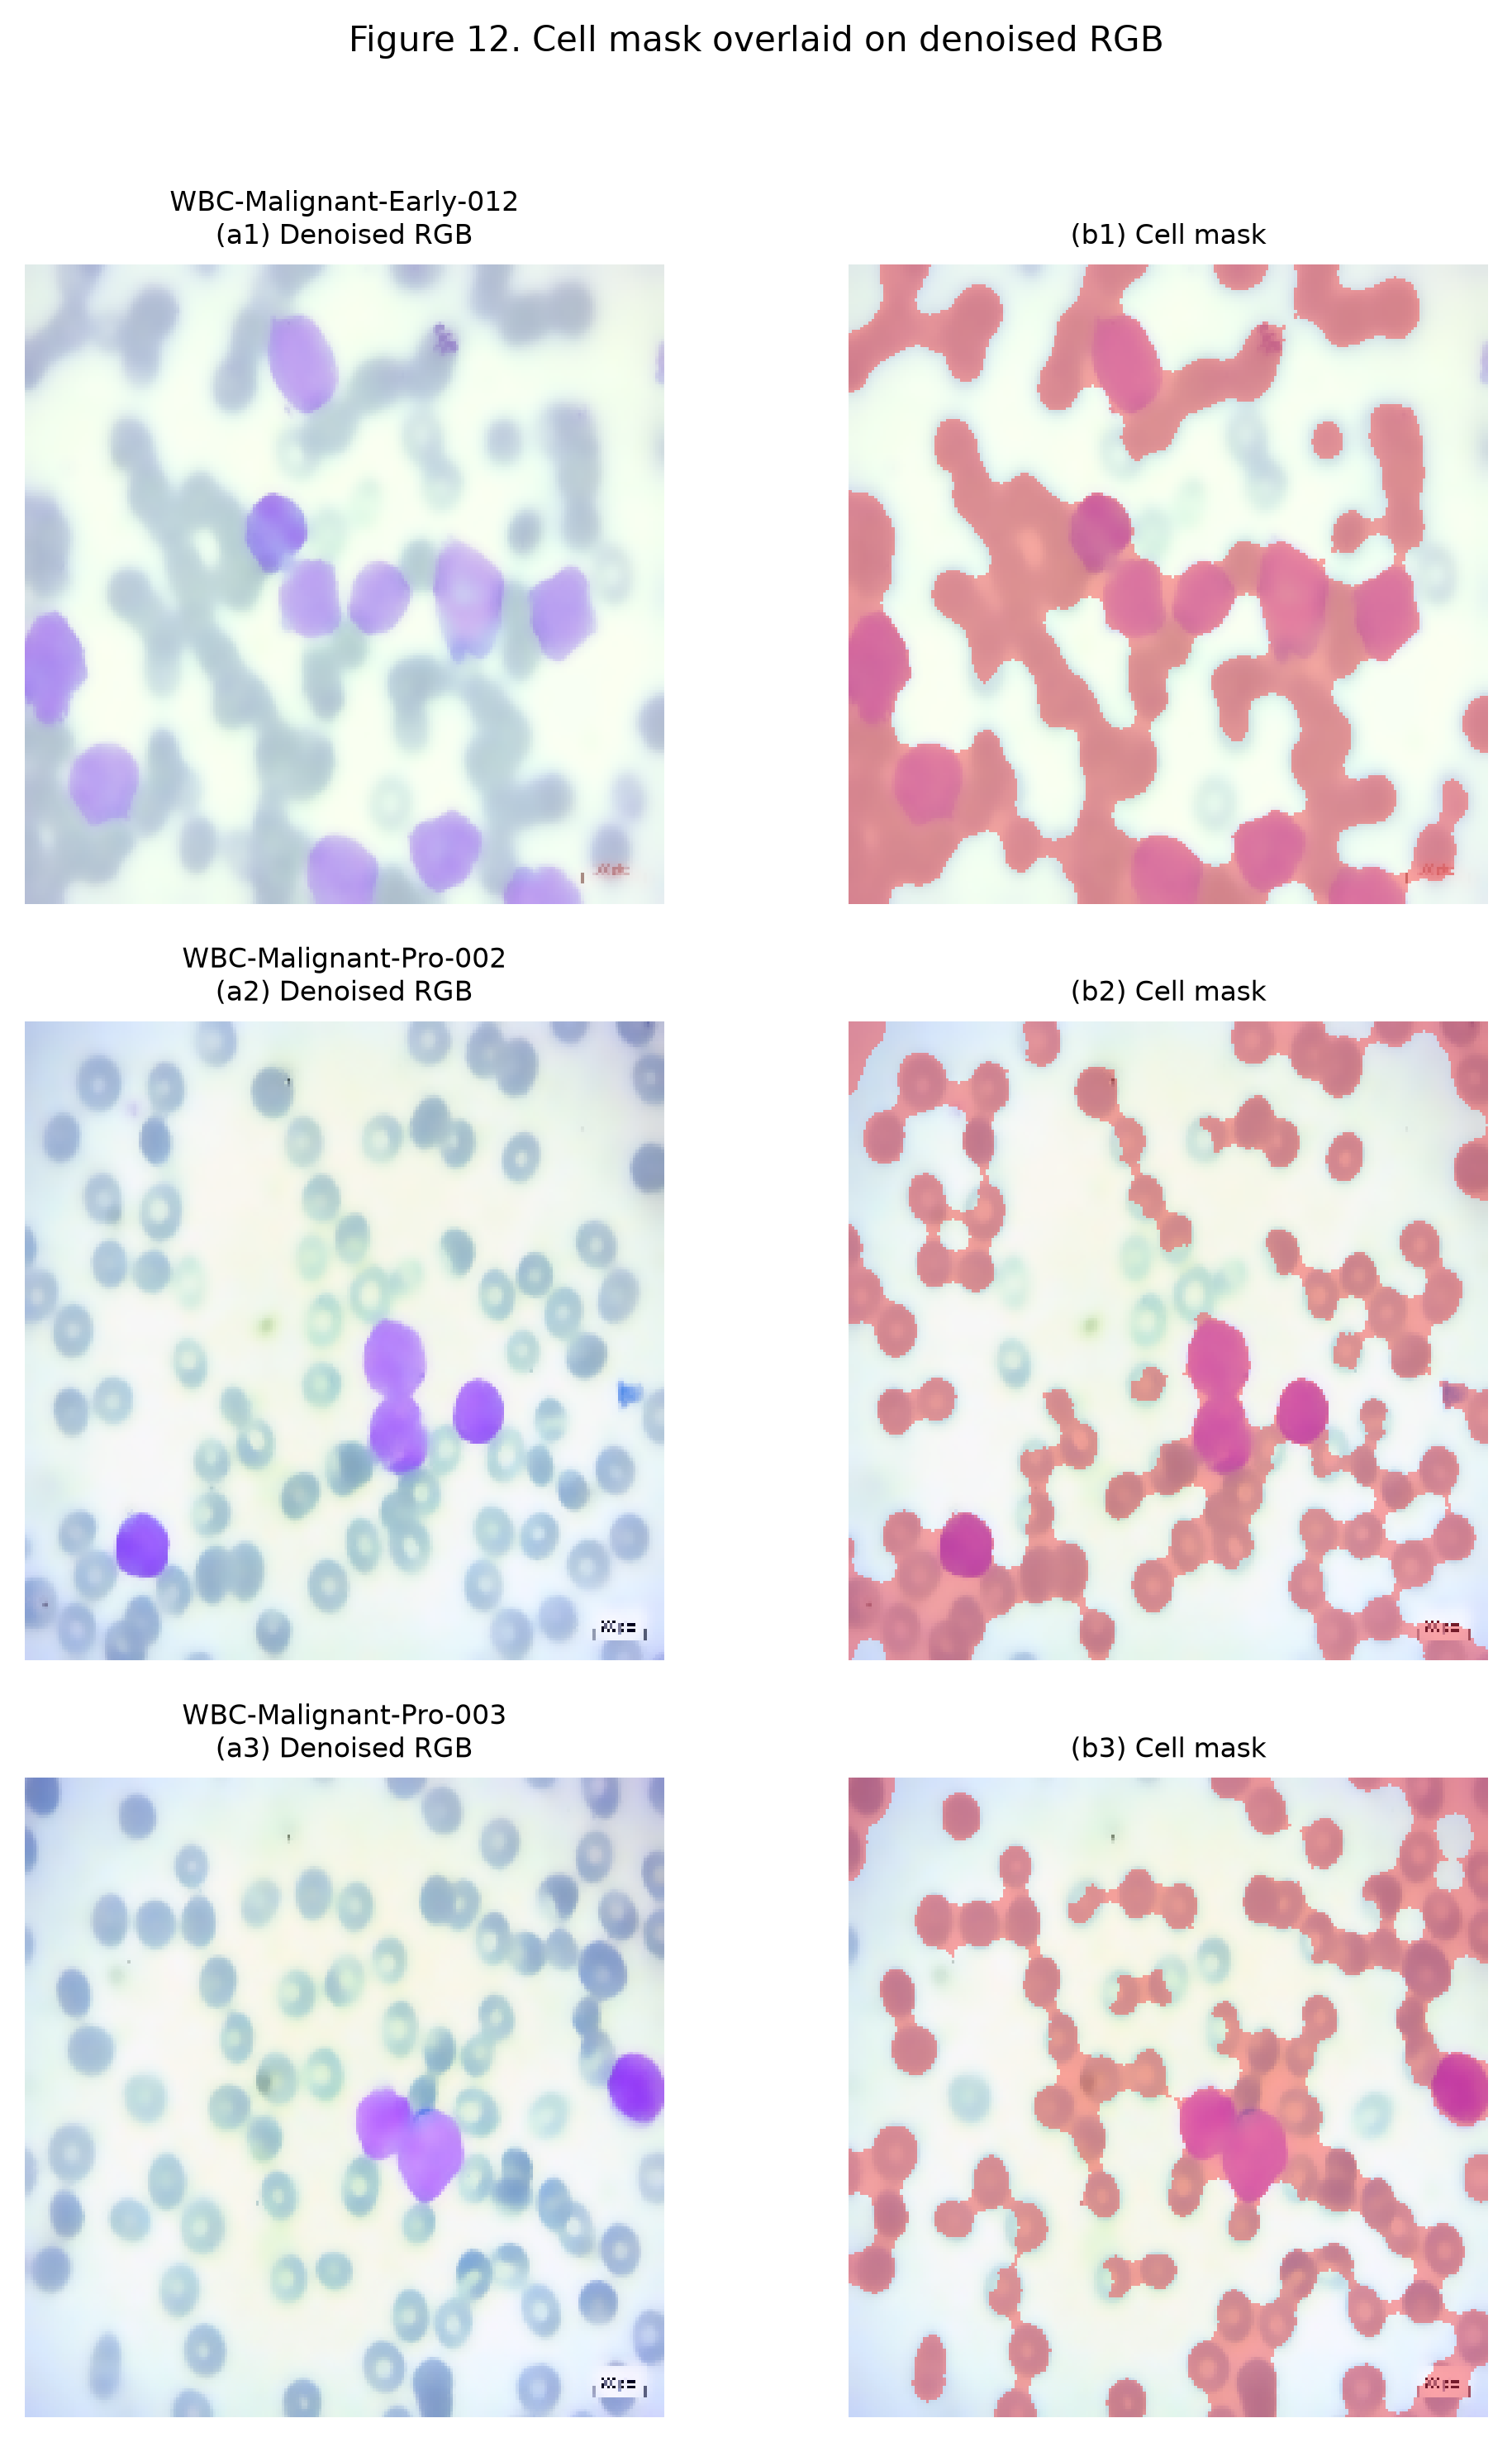
\includegraphics[width=\linewidth]{fig12_cell_overlay.png}
  \caption{Cell mask (translucent red overlay) on the three demo images. Both WBCs and erythrocytes are captured; distinguishing them requires additional cues.}
  \label{fig:cellseg}
\end{figure}

% ------------------------------------------------------------------
\subsection{Nucleus Segmentation (Otsu-within-cell)}
\label{sec:nucseg}

\paragraph{Purpose.} Isolate the deeply-stained purple nuclei from the surrounding lighter cytoplasm --- the primary morphological substrate for leukemia grading.

\paragraph{Method.} A second Otsu threshold $\tau^{**}$ is computed on the \emph{intensities of pixels inside} $M_{\mathrm{cell}}$ only. The nucleus mask is
\begin{equation}
  M_{\mathrm{nuc}}(x) = \mathbb{1}[g(x) < \tau^{**}] \wedge M_{\mathrm{cell}}(x),
\end{equation}
followed by closing with $r_n = 3$ and the same small-component filter.

\paragraph{Rationale.} Restricting Otsu to cell interiors removes the confounding influence of the pale background on the threshold. It also enforces the biological constraint that a nucleus lies within a cell.

\paragraph{Diagnostic behaviour.} Figure~\ref{fig:nucseg} shows the nucleus mask as a translucent blue overlay. Anucleate erythrocytes are correctly ignored --- their interiors are not sufficiently darker than their cytoplasm-free centres to cross the within-cell Otsu threshold --- and only the WBC nuclei light up. This is the property that makes the pipeline diagnostically meaningful.

\begin{figure}[t]
  \centering
  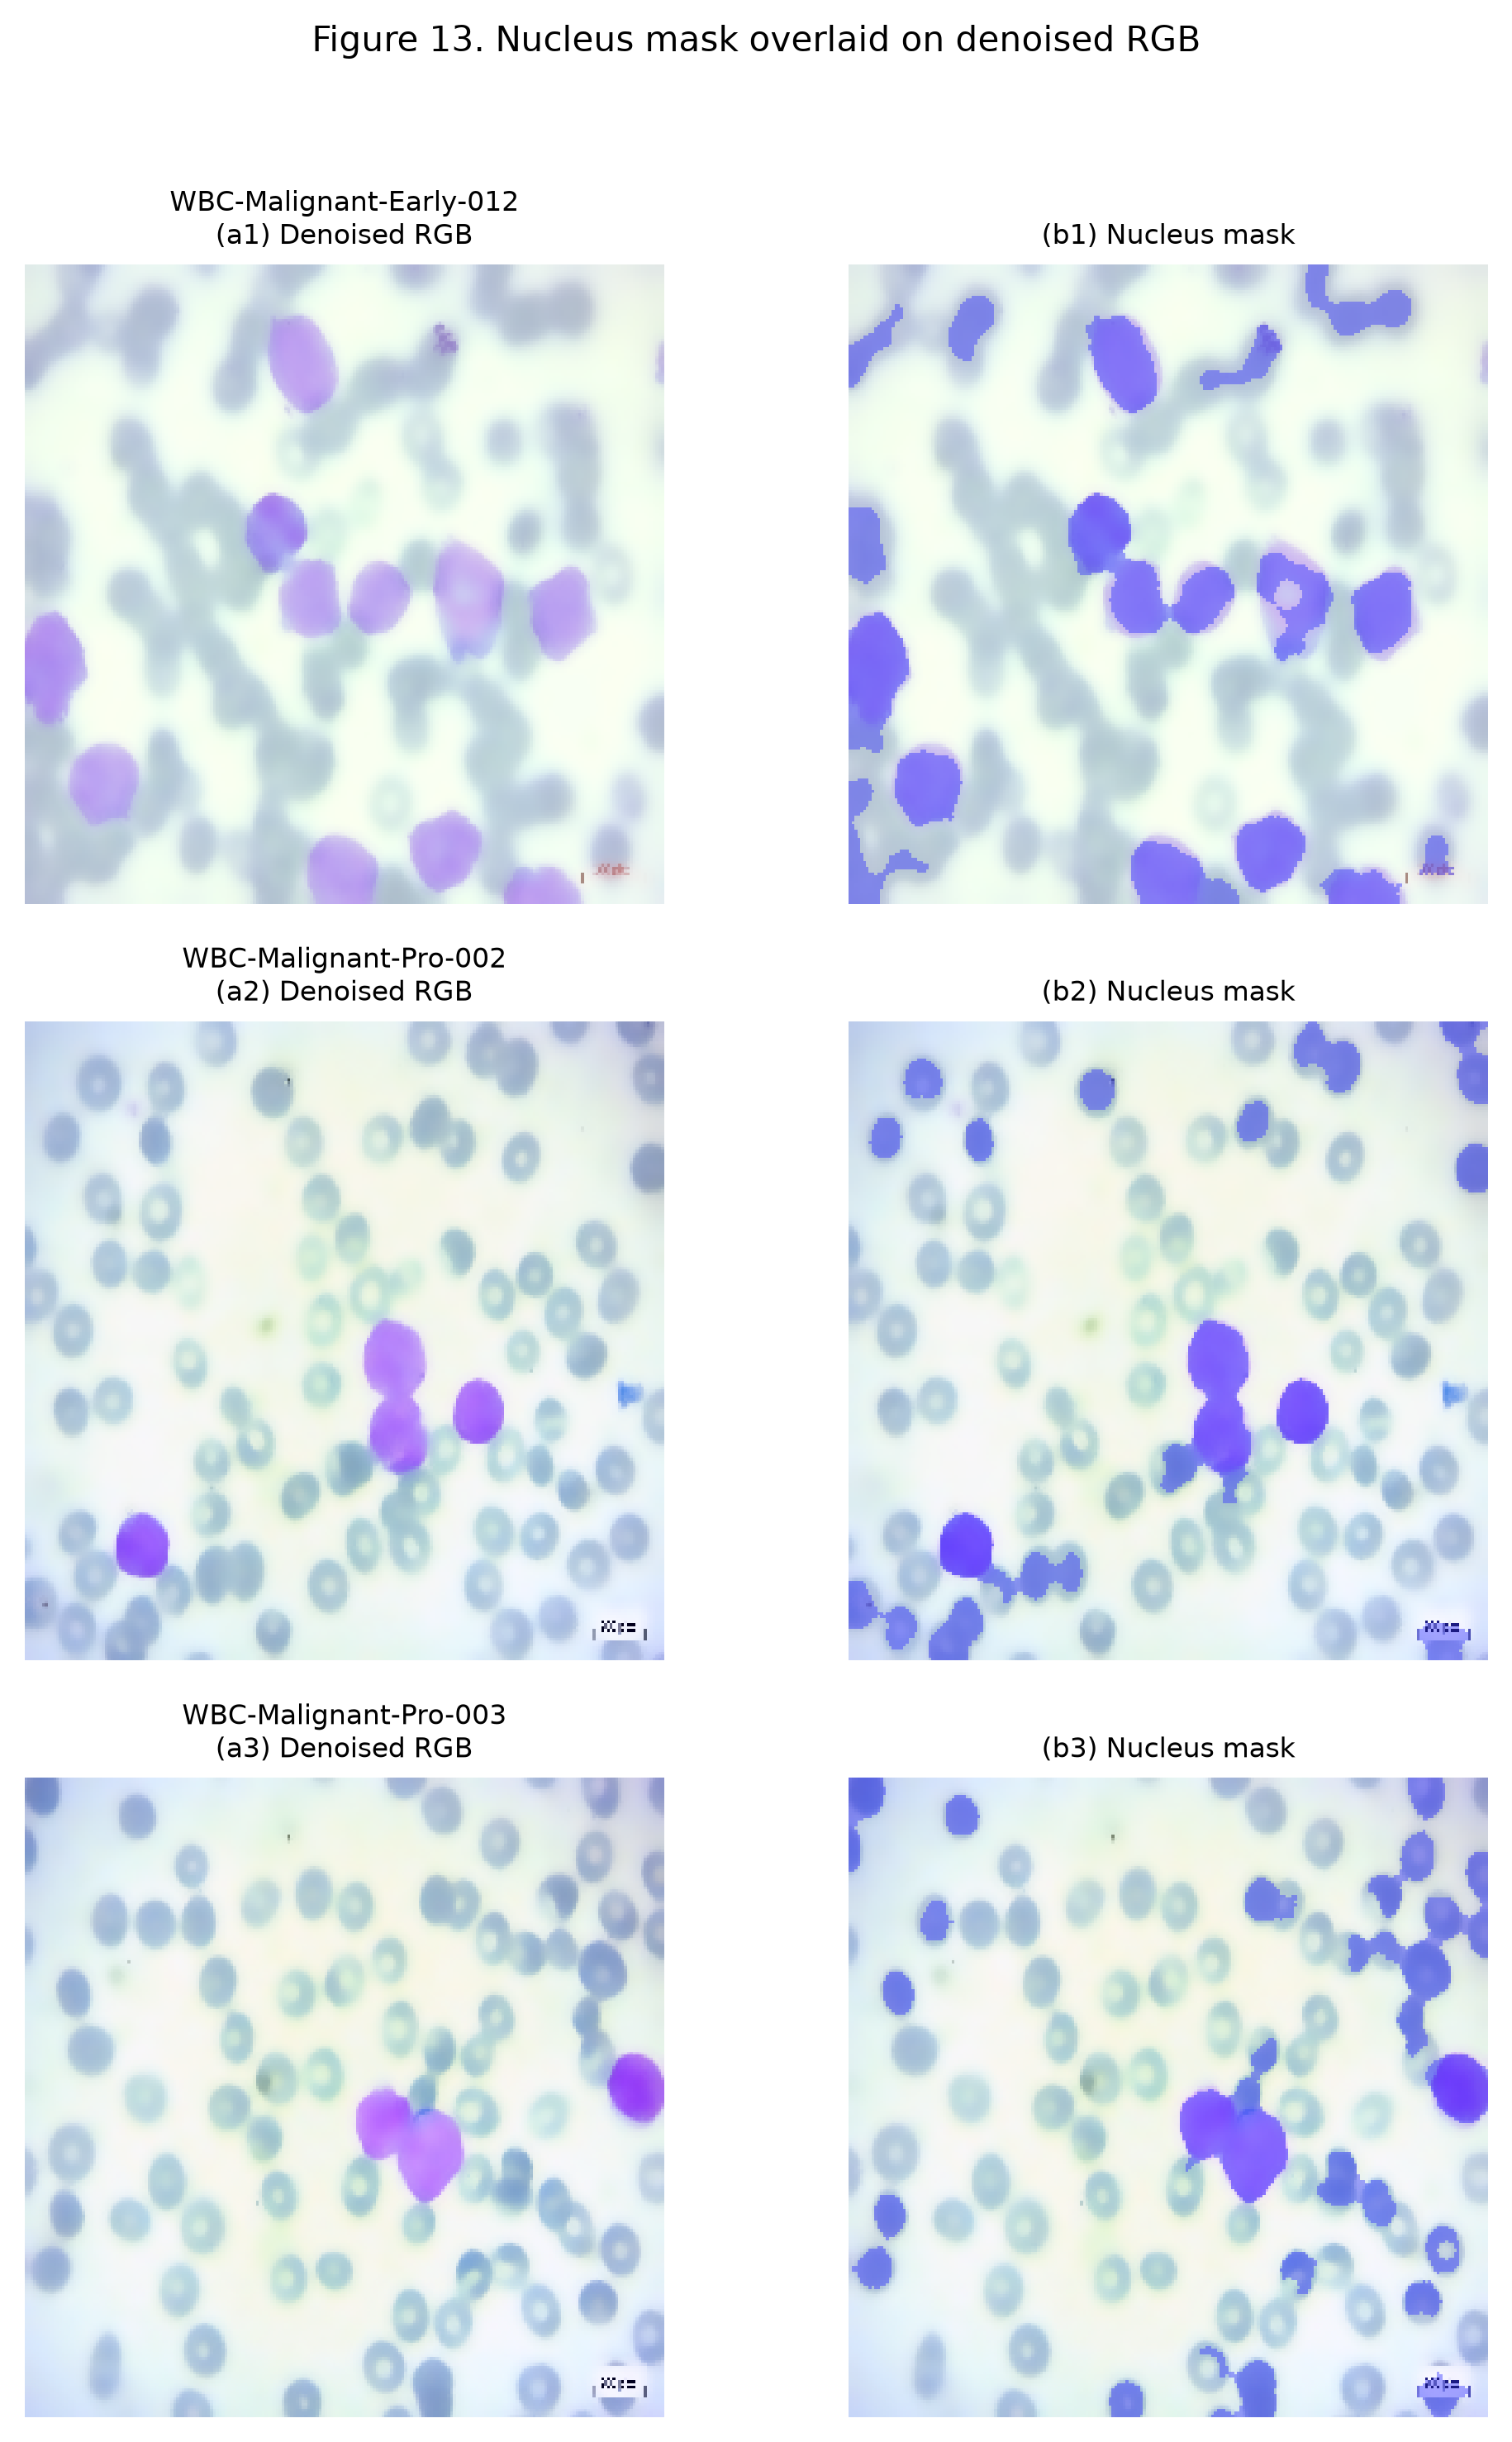
\includegraphics[width=\linewidth]{fig13_nucleus_overlay.png}
  \caption{Nucleus mask (translucent blue overlay). Only WBC nuclei are captured; anucleate erythrocytes are correctly ignored.}
  \label{fig:nucseg}
\end{figure}

% ==================================================================
\section{Feature Extraction}
\label{sec:features}

Fifteen per-image features are extracted (Table~\ref{tab:features}). These populate a single row of \texttt{features.csv} suitable as input to classical machine learning models (support vector machines, gradient-boosted trees).

\subsection{Morphology}
For each connected component in a binary mask $M$, the \texttt{skimage.measure.regionprops} routine returns area $A_r$, perimeter $P_r$, eccentricity $e_r \in [0,1]$ (ratio of focal distance to major-axis length), and solidity $s_r$ (ratio of component area to convex-hull area). We aggregate across components because a single image can contain multiple cells:
\begin{align}
  A_M &= \sum_r A_r, \qquad P_M = \sum_r P_r, \\
  \bar{e}_M &= \frac{1}{|R|}\sum_r e_r, \qquad
  \bar{s}_M = \frac{1}{|R|}\sum_r s_r.
\end{align}
The nuclear-to-cytoplasmic (N/C) ratio is a scalar composite of the two masks:
\begin{equation}
  \mathrm{N/C} = \frac{A_{M_{\mathrm{nuc}}}}{A_{M_{\mathrm{cell}}}}.
  \label{eq:ncratio}
\end{equation}
Elevated N/C is a classical marker of malignant lymphoblasts, whose nuclei can occupy 90\% of the cell interior.

\subsection{Texture (GLCM)}
The gray-level co-occurrence matrix $P(i, j \mid d, \theta)$ counts pairs of pixels with intensities $i, j$ separated by displacement $(d, \theta)$. We use $d = 1$, $\theta = 0$ (horizontal), 256 levels, and the four Haralick descriptors:
\begin{align}
  \mathrm{Contrast}    &= \sum_{i,j} (i - j)^2 P(i, j) \\
  \mathrm{Energy}      &= \sqrt{\sum_{i,j} P(i, j)^2} \\
  \mathrm{Homogeneity} &= \sum_{i,j} \frac{P(i, j)}{1 + |i - j|} \\
  \mathrm{Correlation} &= \sum_{i,j} \frac{(i - \mu_i)(j - \mu_j) P(i, j)}{\sigma_i \sigma_j}
\end{align}
Chromatin coarseness (relevant for leukemia grading) manifests as elevated contrast and depressed homogeneity.

\subsection{Colour statistics}
Per-channel mean and standard deviation of the denoised RGB image (six scalars). These capture the residual colour signature not eliminated by stain normalization.

\begin{table}[t]
  \centering
  \caption{Feature vector columns.}
  \label{tab:features}
  \small
  \begin{tabular}{@{}ll@{}}
    \toprule
    Category & Columns \\
    \midrule
    Identity   & \texttt{image\_id}, \texttt{class\_name}, \texttt{split} \\
    Labels     & \texttt{class\_id\_binary}, \texttt{class\_id\_4way} \\
    Morphology & \texttt{nucleus\_\{area,perim,eccentricity,solidity\}} \\
               & \texttt{cell\_area}, \texttt{nc\_ratio} \\
    Texture    & \texttt{glcm\_\{contrast,energy,homogeneity,correlation\}} \\
    Colour     & \texttt{mean\_\{R,G,B\}}, \texttt{std\_\{R,G,B\}} \\
    \bottomrule
  \end{tabular}
\end{table}

% ==================================================================
\section{Data Formats}
\label{sec:formats}

Preprocessing writes three artefacts to disk:

\subsection{Per-image \texttt{.npz} tensor}
Located at \texttt{data/cache/\{split\}/\{image\_id\}.npz}. Contains six arrays:
\begin{lstlisting}
rgb          (H, W, 3)  uint8
apc          (H, W)     float32   in [0, 1]
log          (H, W)     float32   in [0, 1]
canny        (H, W)     bool
nucleus_mask (H, W)     bool
cell_mask    (H, W)     bool
\end{lstlisting}
At training time a PyTorch \texttt{Dataset} stacks whichever channels are desired: e.g., \texttt{concat(rgb, apc, log, canny)} yields a $(H, W, 6)$ input.

\subsection{\texttt{features.csv}}
One row per image, columns as in Table~\ref{tab:features}. Directly loadable as a \texttt{pandas.DataFrame} for classical models.

\subsection{\texttt{manifest.csv}}
The authoritative train/val/test split. Columns: \texttt{image\_id}, \texttt{orig\_path}, \texttt{class\_name}, \texttt{class\_id\_binary}, \texttt{class\_id\_4way}, \texttt{split}. The split is stratified per class with a fixed random seed to ensure reproducibility across runs.

% ==================================================================
\section{Worked Examples}
\label{sec:demo}

We demonstrate the pipeline on three images drawn from the Aria dataset: one Early~Pre-B (\texttt{Early-012}) and two Pro-B (\texttt{Pro-002}, \texttt{Pro-003}). Figures~\ref{fig:full1}--\ref{fig:full3} show all six output layers for each image; Figures~\ref{fig:flow1}--\ref{fig:flow3} present the same information as a seven-panel pipeline strip highlighting the flow from raw input to final segmentation. Table~\ref{tab:featvals} lists the extracted feature values.

\begin{figure}[t]
  \centering
  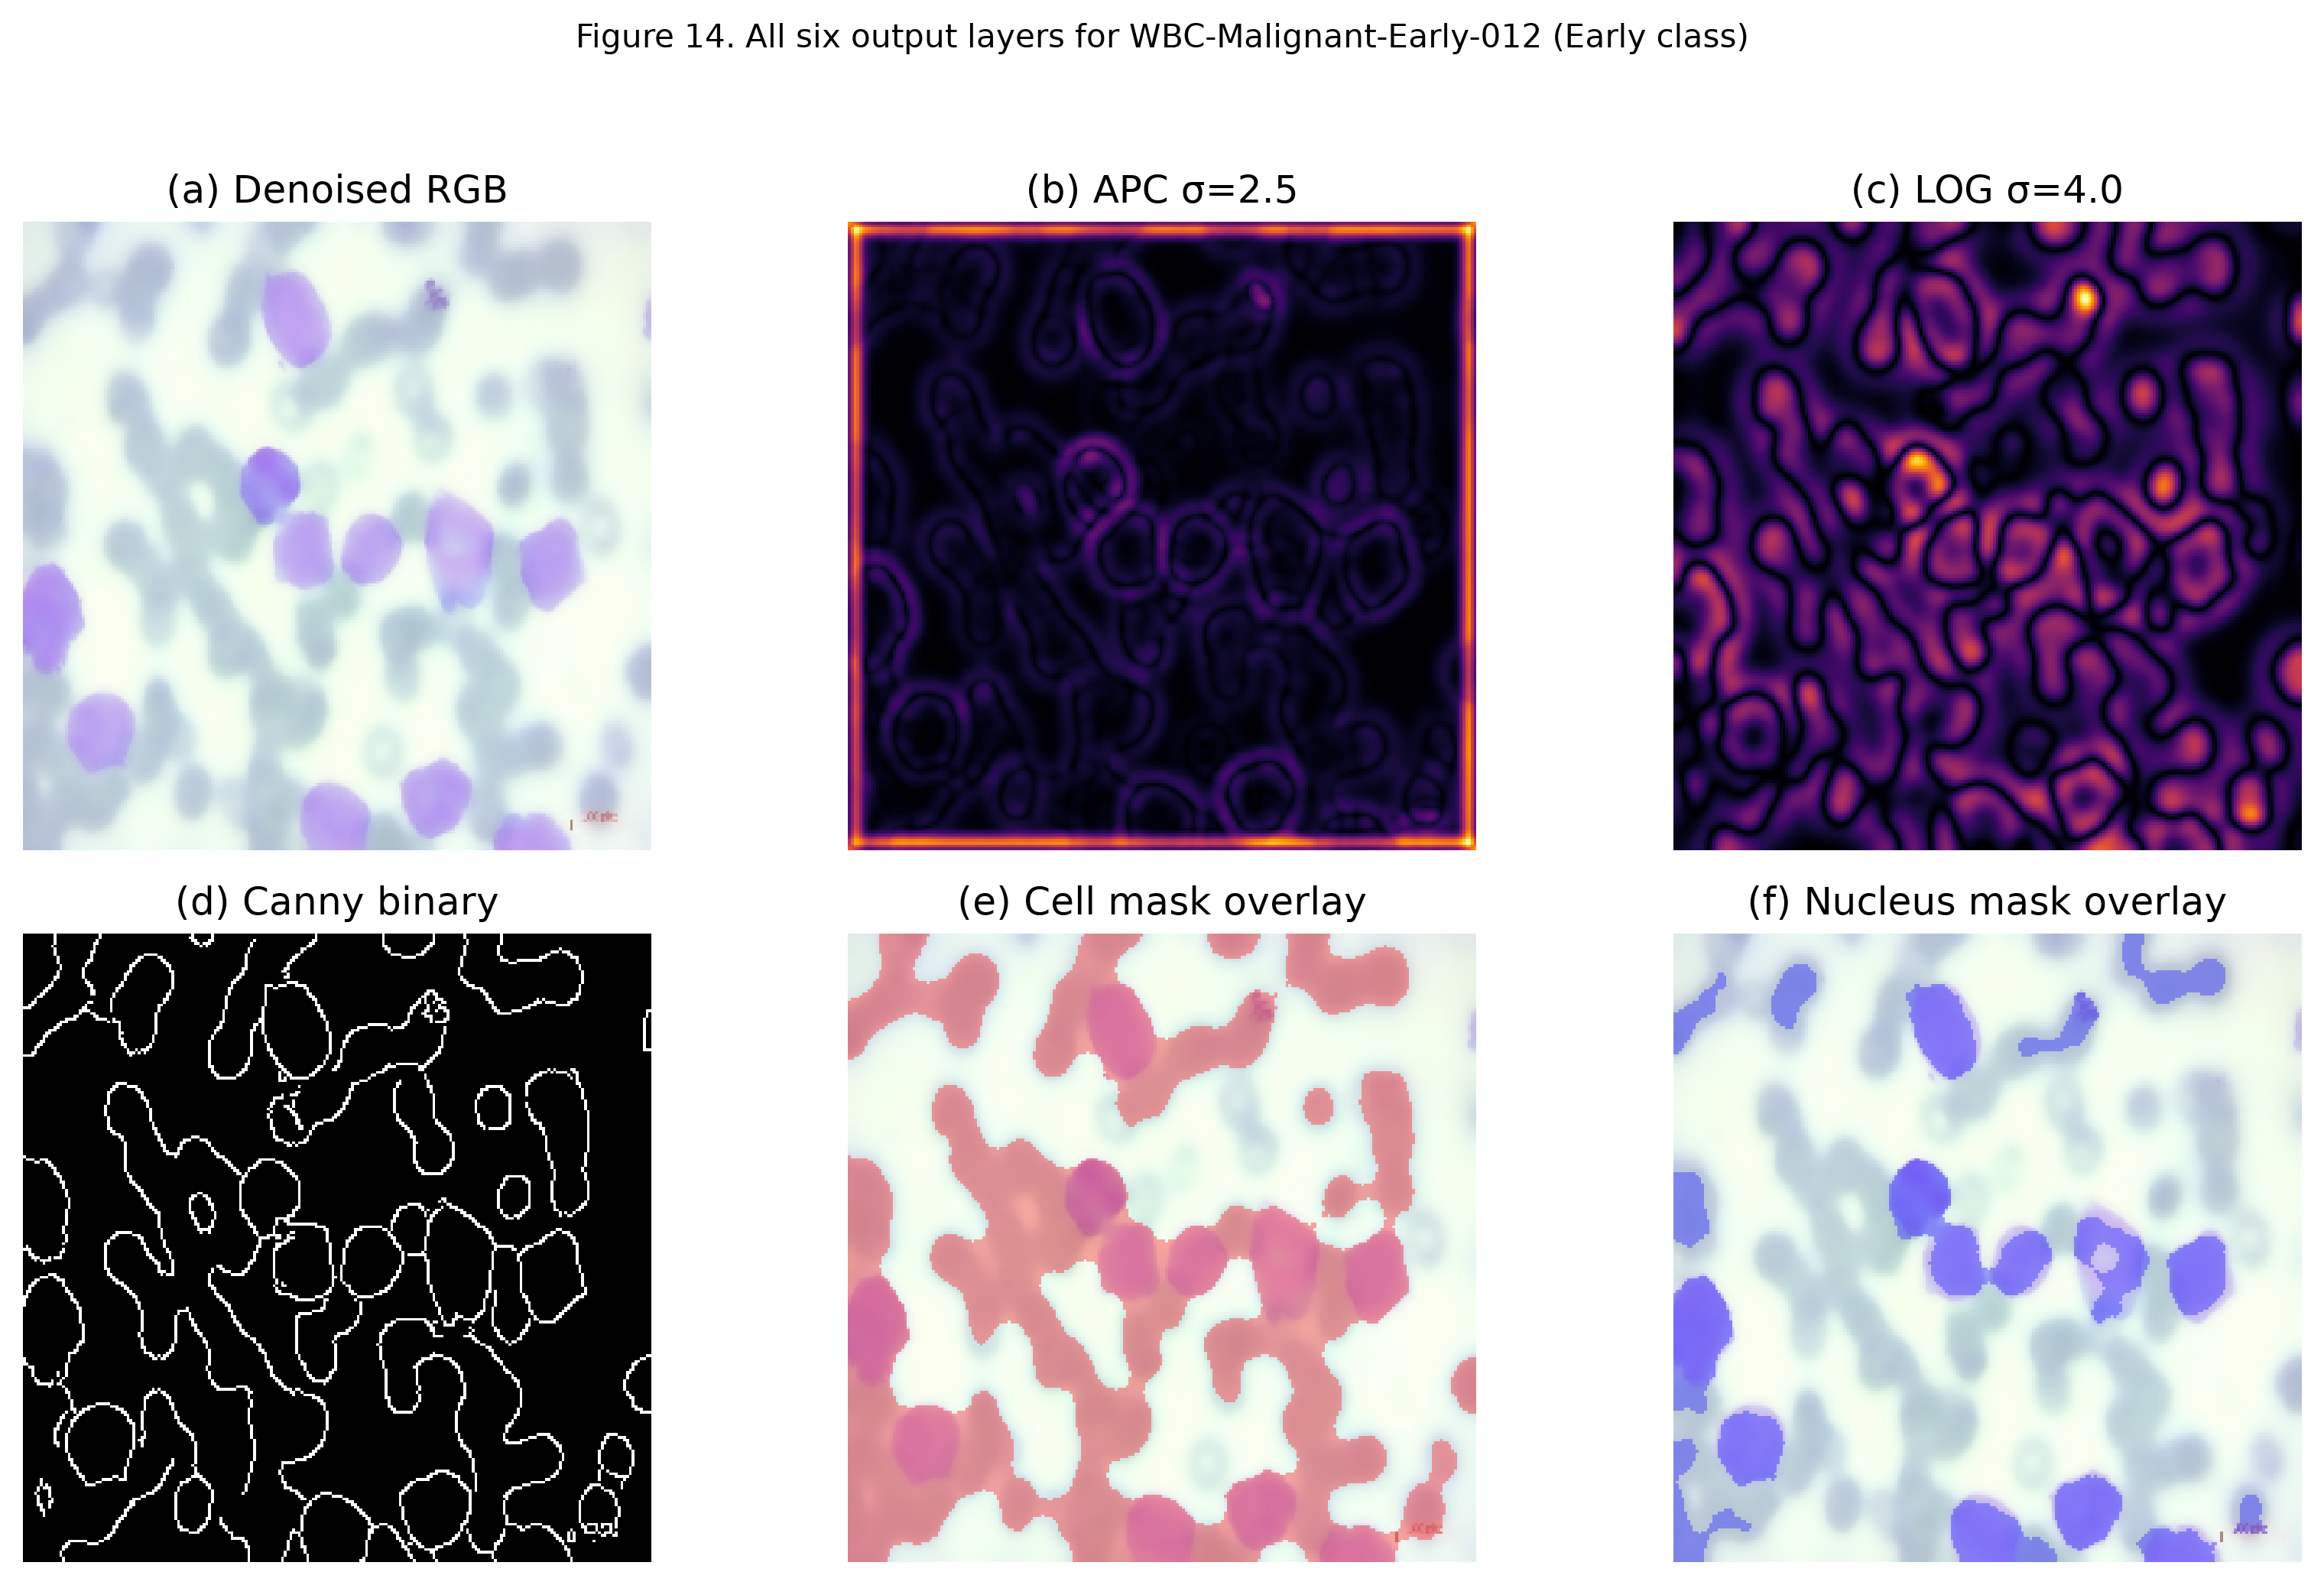
\includegraphics[width=\linewidth]{fig14_full_early012.png}
  \caption{All six output layers for \texttt{WBC-Malignant-Early-012} (Early Pre-B class). Multiple WBCs are present; the nucleus mask captures each purple region.}
  \label{fig:full1}
\end{figure}

\begin{figure}[t]
  \centering
  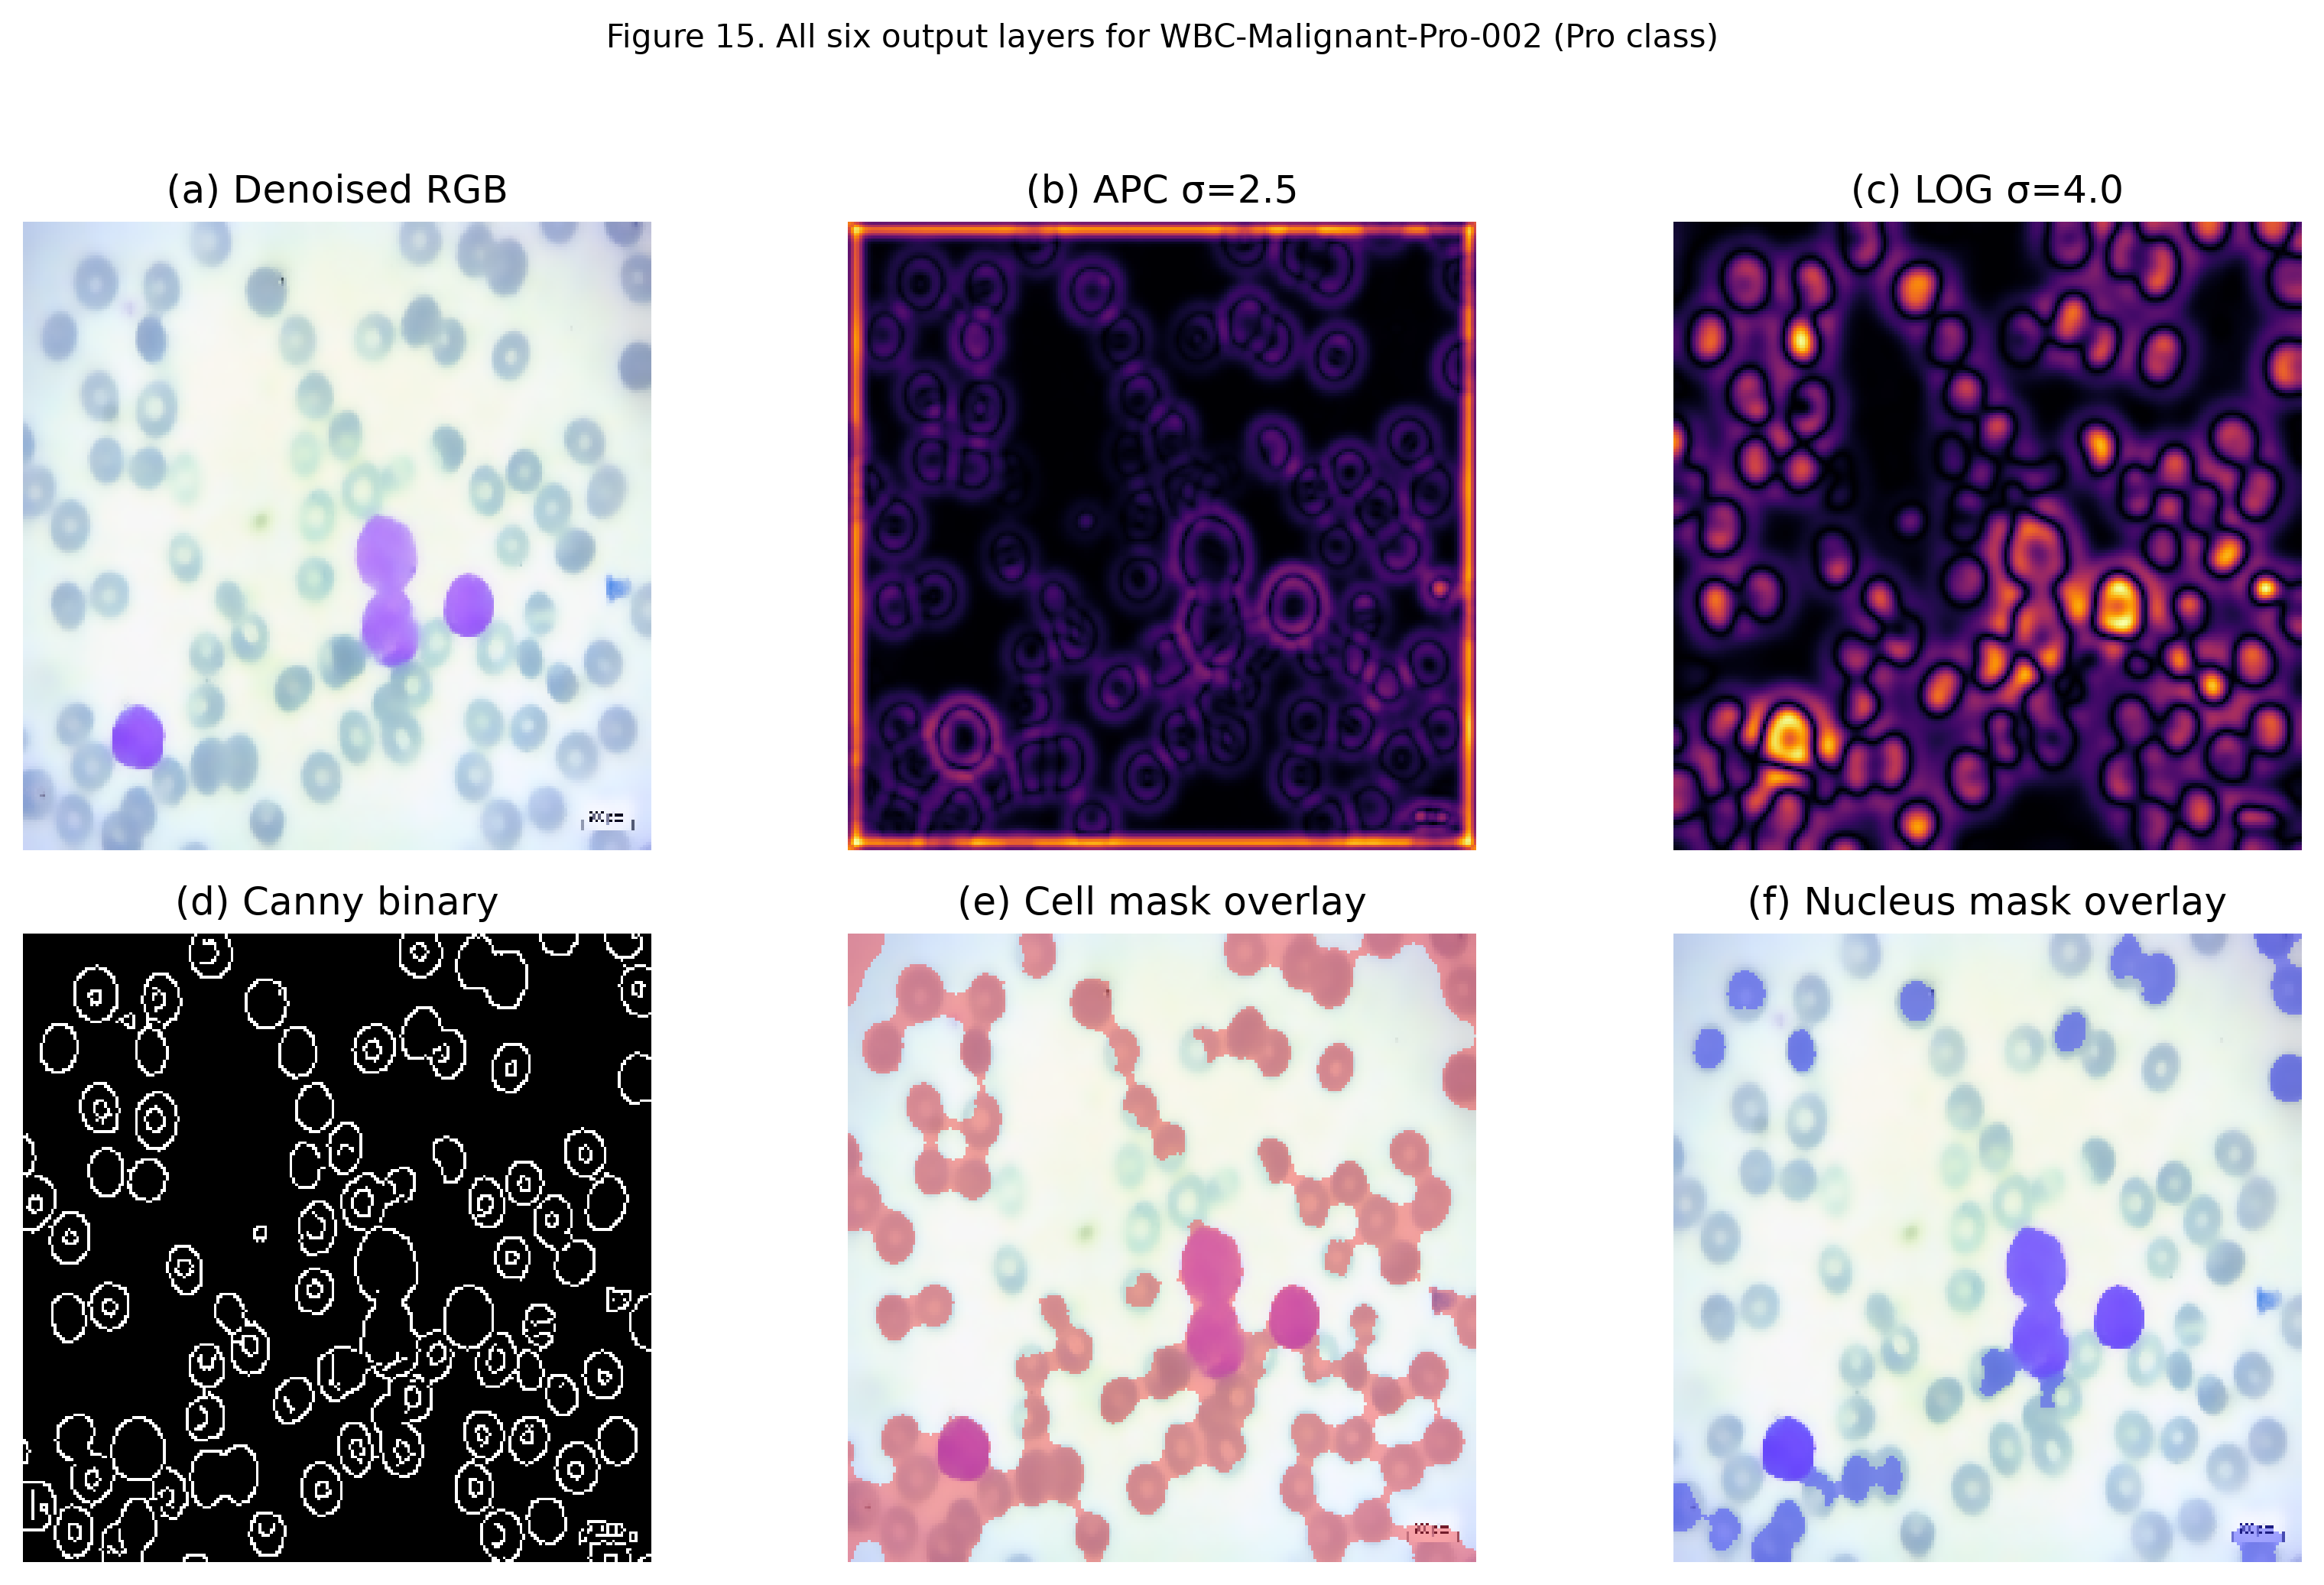
\includegraphics[width=\linewidth]{fig15_full_pro002.png}
  \caption{All six output layers for \texttt{WBC-Malignant-Pro-002} (Pro-B class, test split). Three WBCs are correctly isolated among a dense erythrocyte background.}
  \label{fig:full2}
\end{figure}

\begin{figure}[t]
  \centering
  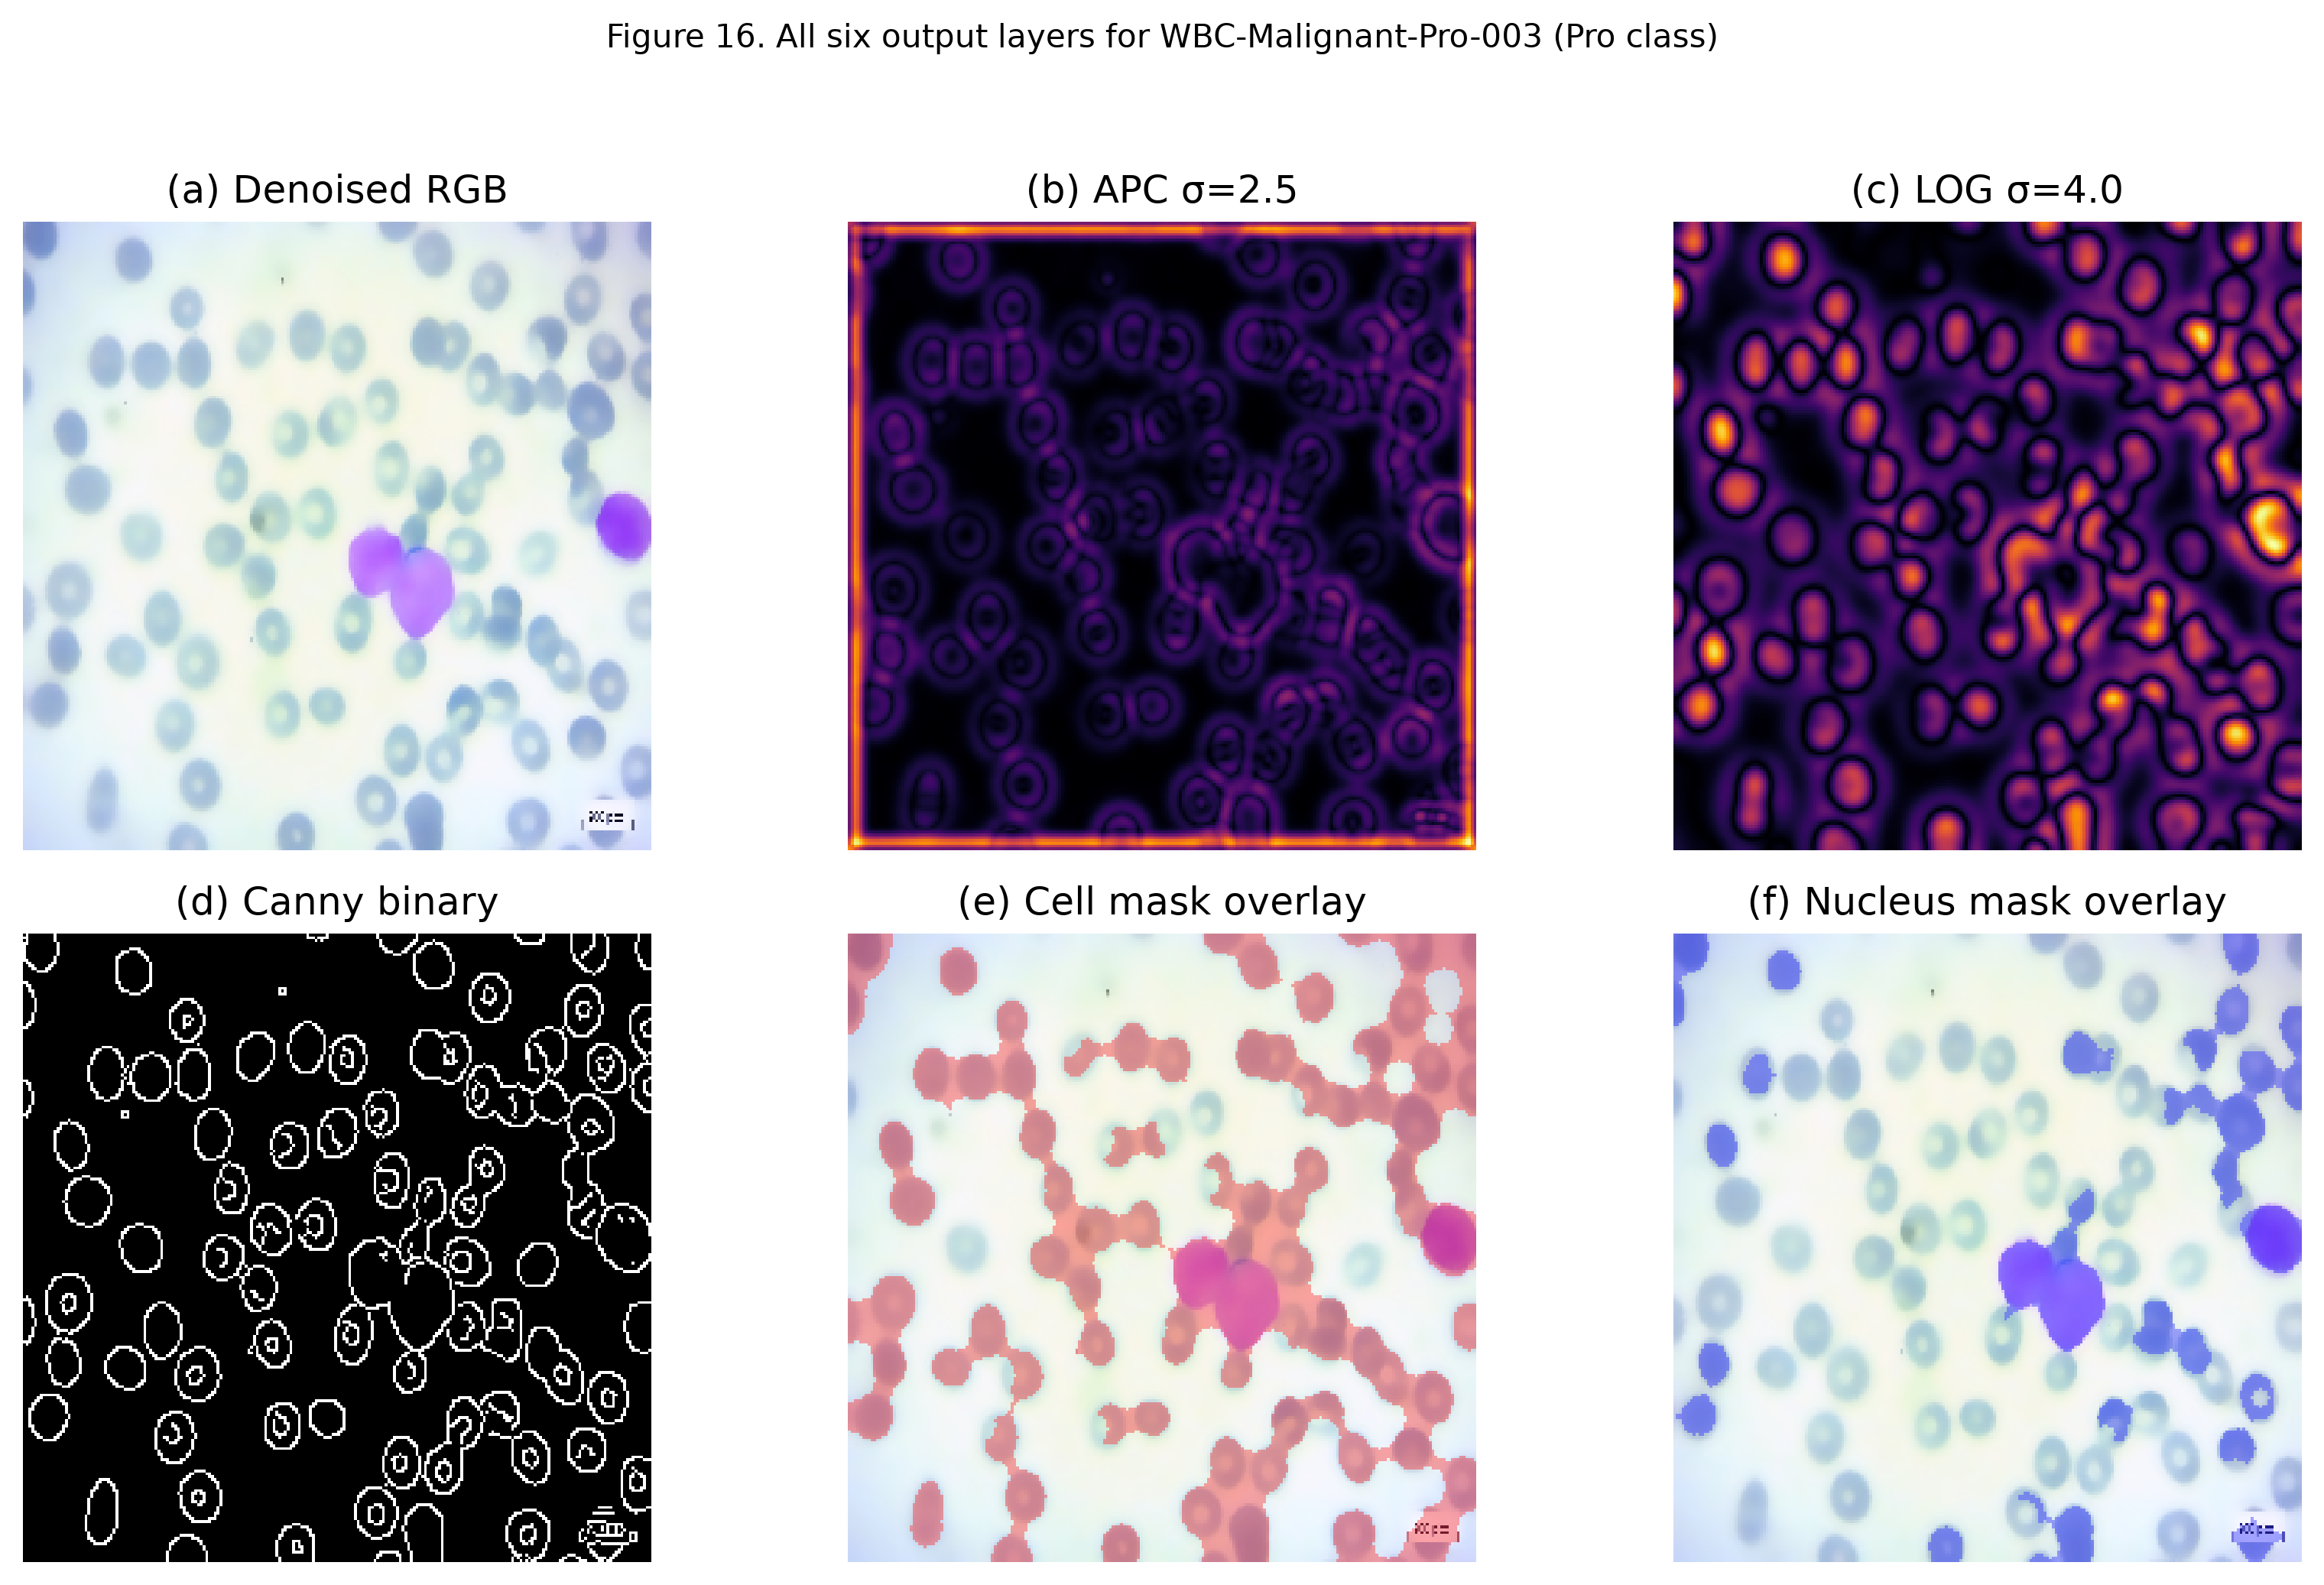
\includegraphics[width=\linewidth]{fig16_full_pro003.png}
  \caption{All six output layers for \texttt{WBC-Malignant-Pro-003} (Pro-B class). Two large purple-stained WBCs dominate the field.}
  \label{fig:full3}
\end{figure}

\begin{figure*}[t]
  \centering
  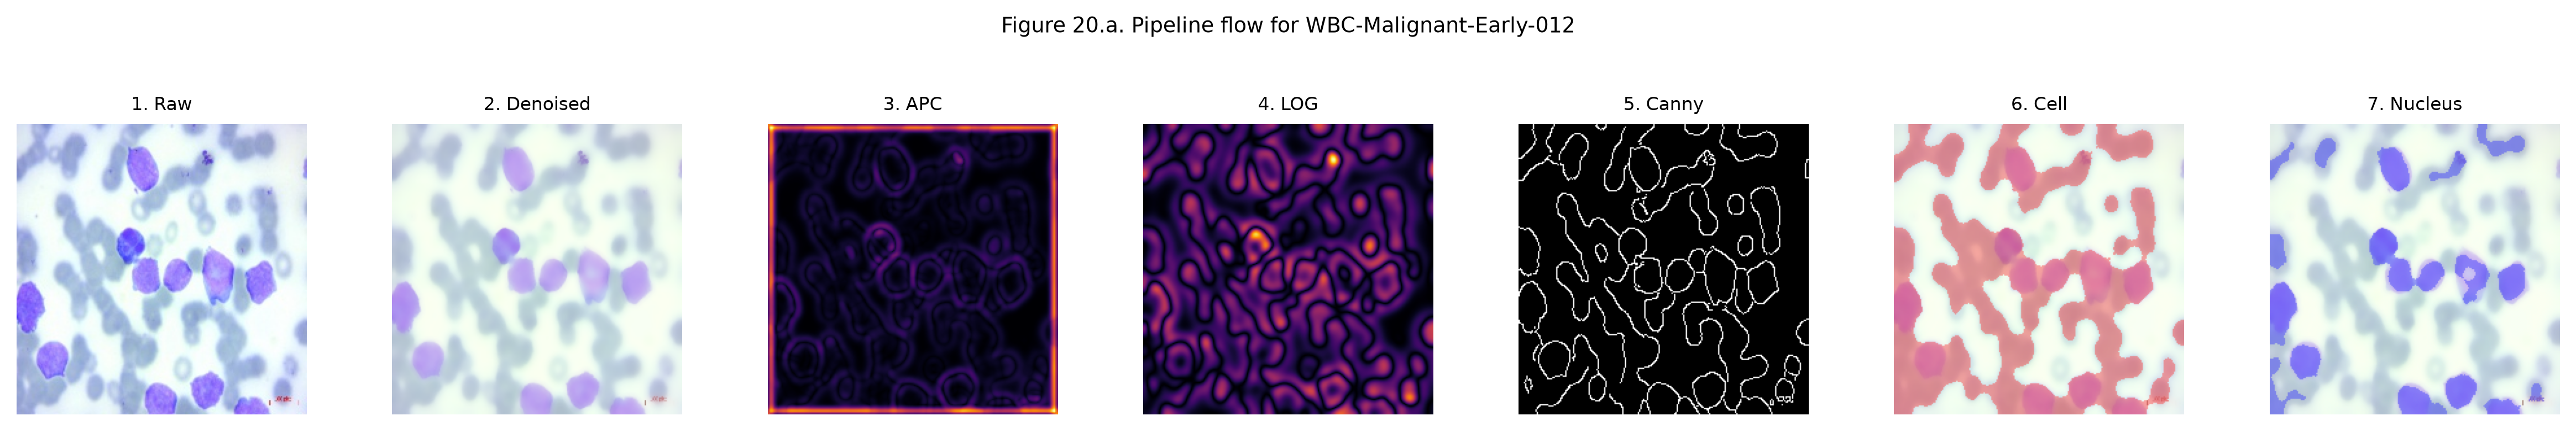
\includegraphics[width=\linewidth]{fig20a_flow_early_012.png}
  \caption{Pipeline flow for Early-012 from raw JPEG through to nucleus overlay.}
  \label{fig:flow1}
\end{figure*}

\begin{figure*}[t]
  \centering
  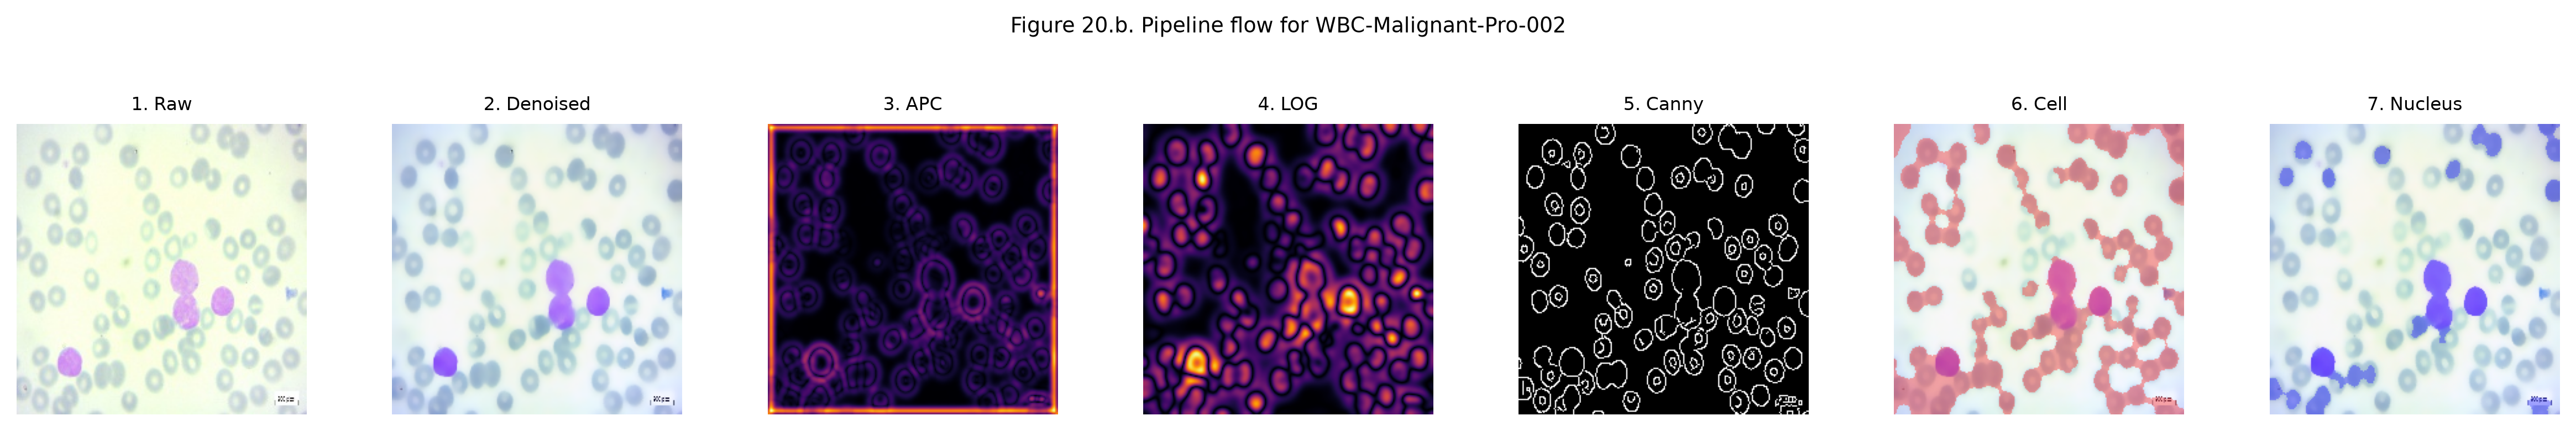
\includegraphics[width=\linewidth]{fig20b_flow_pro_002.png}
  \caption{Pipeline flow for Pro-002.}
  \label{fig:flow2}
\end{figure*}

\begin{figure*}[t]
  \centering
  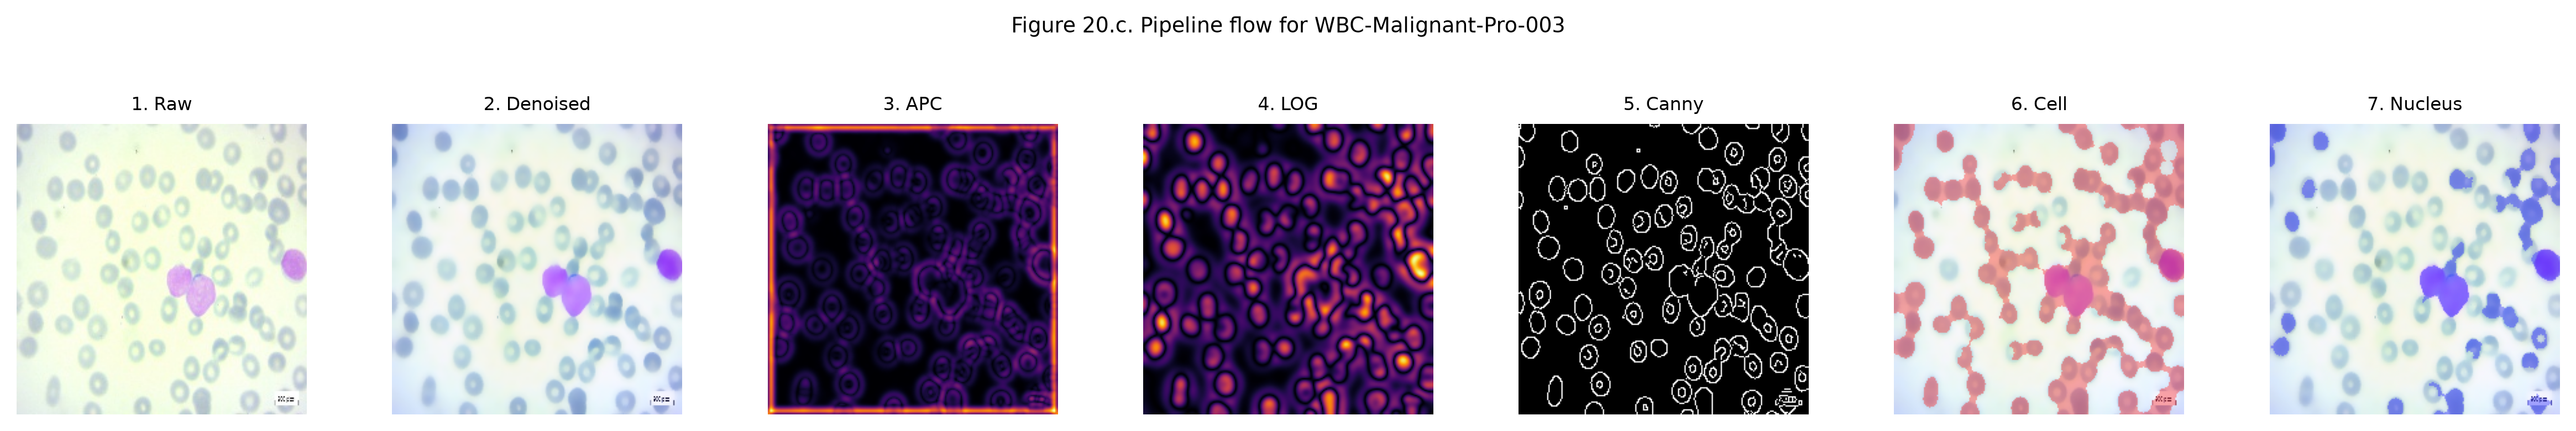
\includegraphics[width=\linewidth]{fig20c_flow_pro_003.png}
  \caption{Pipeline flow for Pro-003.}
  \label{fig:flow3}
\end{figure*}

\begin{figure*}[t]
  \centering
  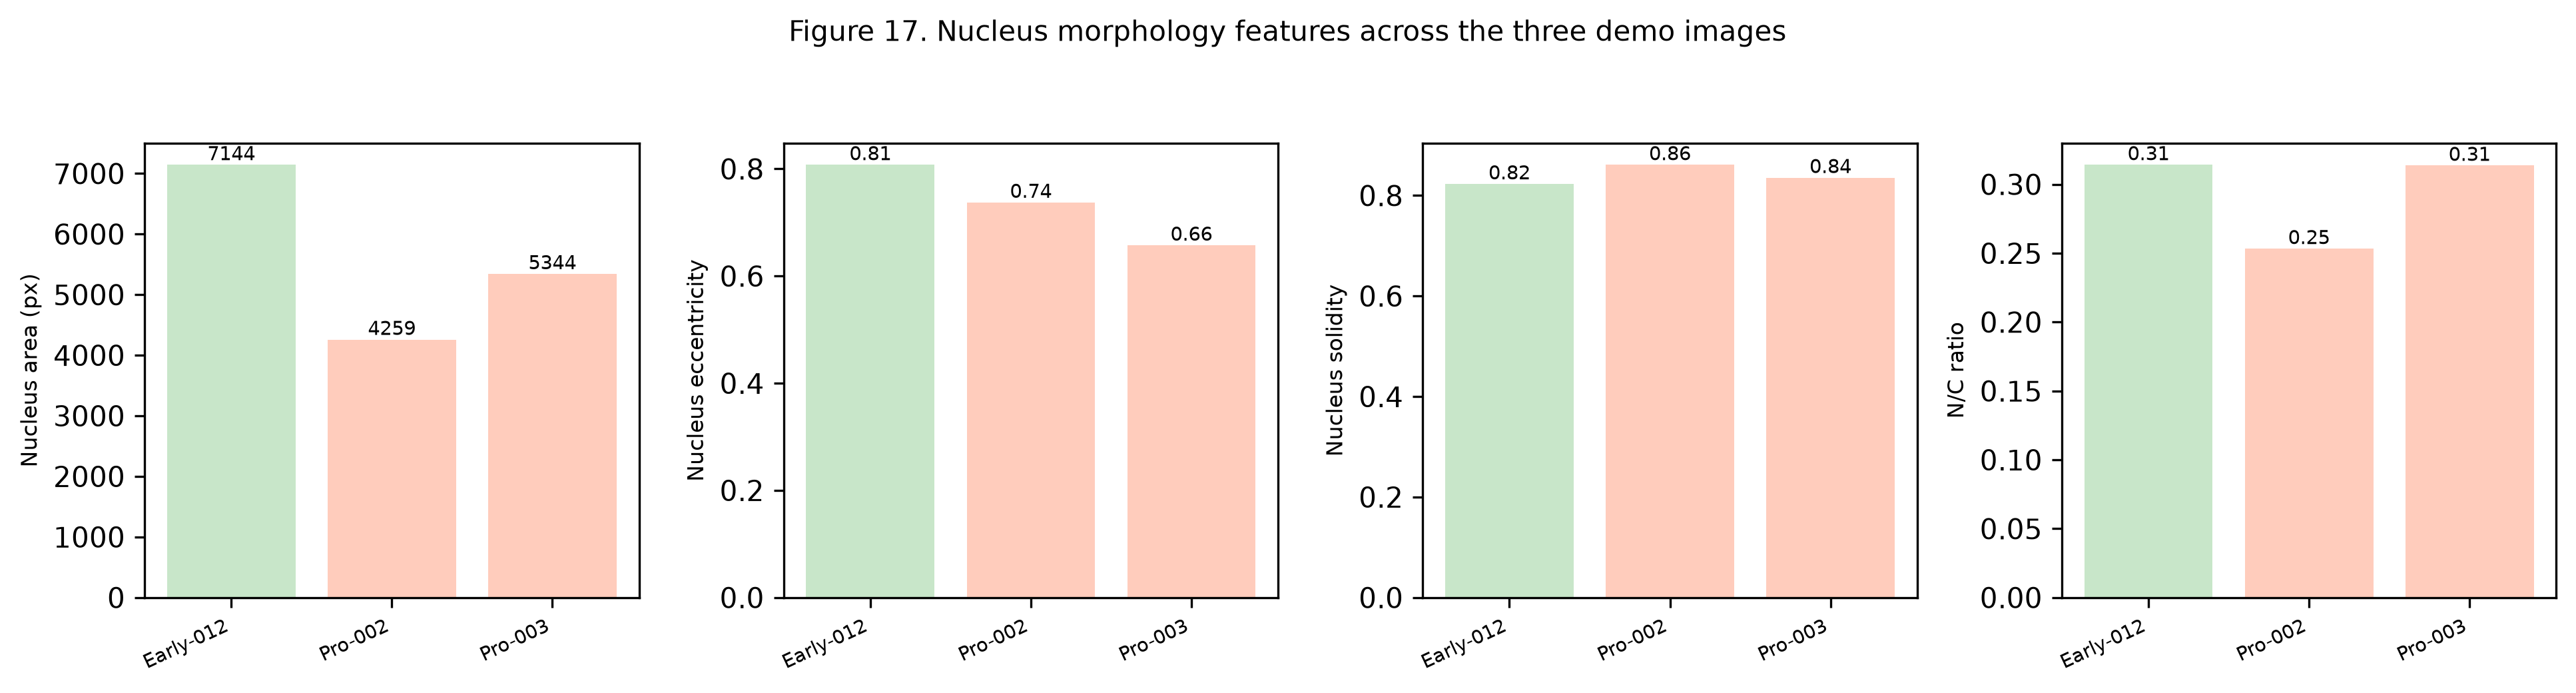
\includegraphics[width=\linewidth]{fig17_morphology_bars.png}
  \caption{Nucleus morphology features across the three demo images. Note the elevated aggregate nucleus area for Early-012 (many small nuclei summed) versus the two Pro-B images (fewer, larger nuclei).}
  \label{fig:morph}
\end{figure*}

\begin{figure*}[t]
  \centering
  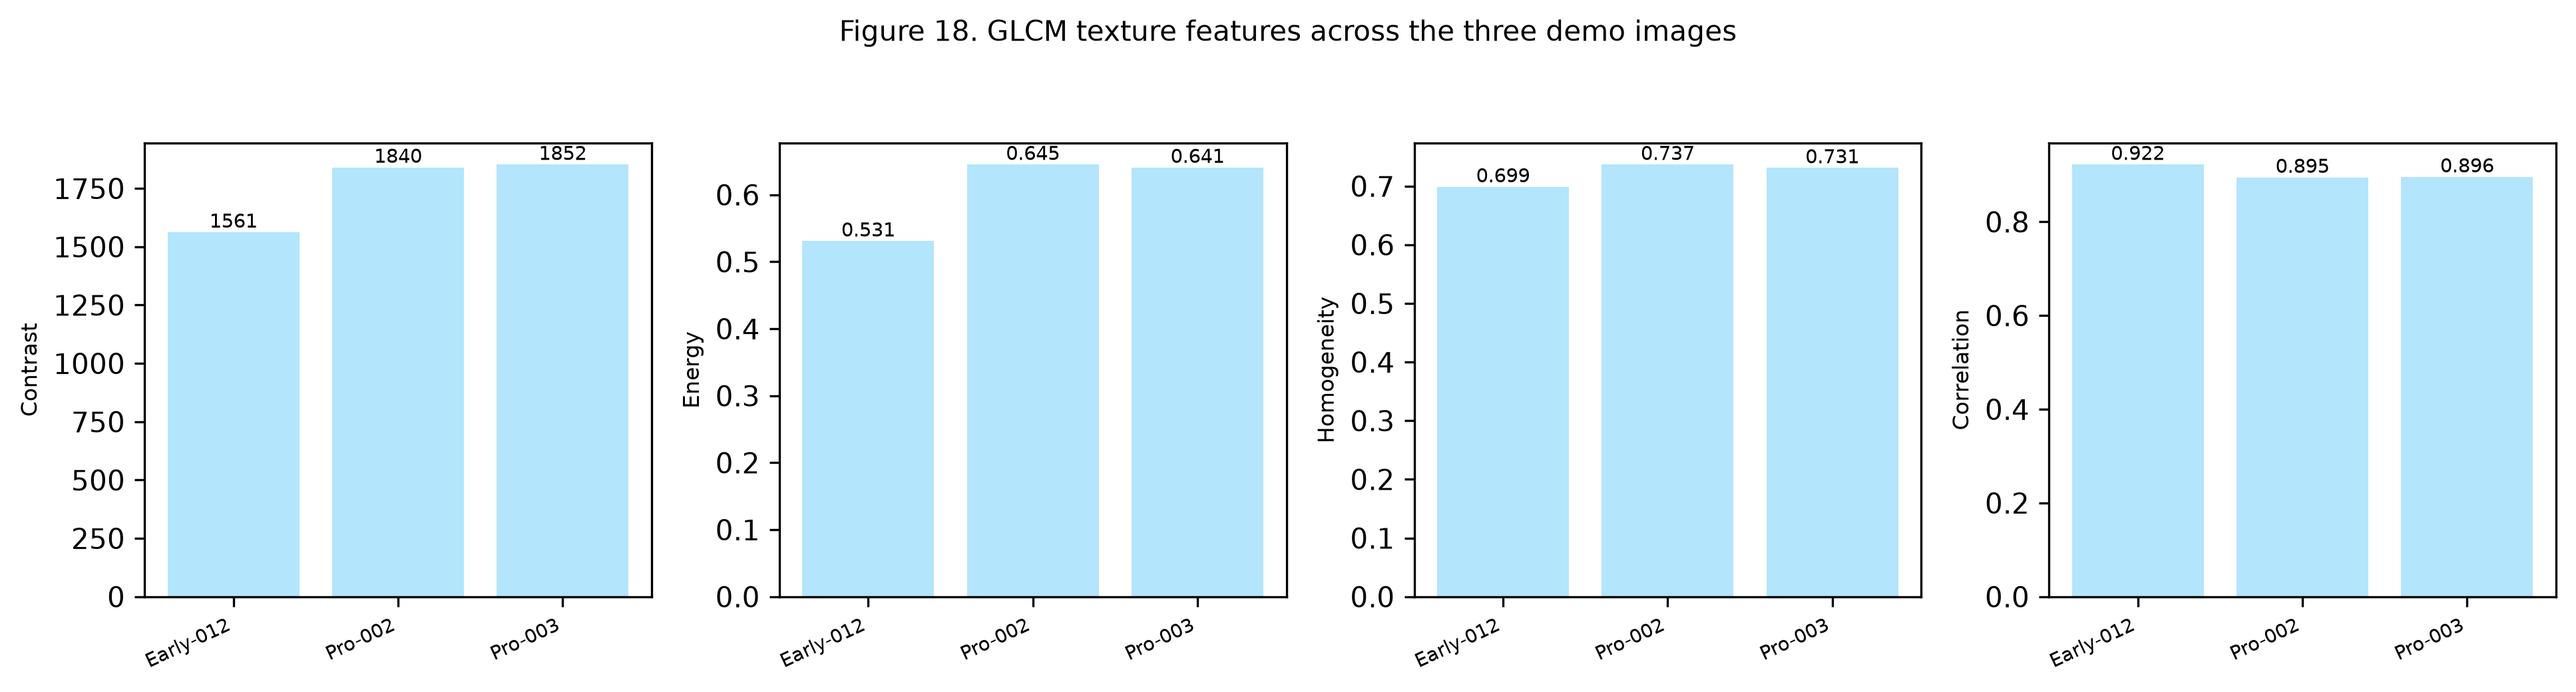
\includegraphics[width=\linewidth]{fig18_glcm_bars.png}
  \caption{GLCM texture features. Pro-003 (largest lymphoblast) shows the lowest energy and highest correlation, consistent with a smoothly stained blast nucleus; Early-012 (many cells, more texture) shows the highest contrast.}
  \label{fig:glcm}
\end{figure*}

\begin{table*}[t]
  \centering
  \caption{Extracted feature values for the three demo images.}
  \label{tab:featvals}
  \small
  \begin{tabular}{@{}lrrrrrrrr@{}}
    \toprule
    Image & Split & Class & Nuc.\ area & Nuc.\ ecc. & Nuc.\ sol. & N/C ratio & GLCM contrast & GLCM energy \\
    \midrule
    Early-012 & train & Early (Pre-B) & 7,144 & 0.808 & 0.823 & 0.314 & 1,562 & 0.093 \\
    Pro-002   & test  & Pro-B         & 4,259 & 0.737 & 0.861 & 0.253 & 1,840 & 0.088 \\
    Pro-003   & train & Pro-B         & 5,344 & 0.657 & 0.835 & 0.314 & 1,852 & 0.089 \\
    \bottomrule
  \end{tabular}
\end{table*}

% ==================================================================
\section{Discussion}
\label{sec:discussion}

\subsection{What works}
The nucleus mask cleanly isolates WBC nuclei from surrounding erythrocytes across all three demonstration images (Fig.~\ref{fig:nucseg}). The APC and LOG response maps are visually informative and align with expected biological structures. Morphological features derived from the nucleus mask (Table~\ref{tab:featvals}) fall in physiologically plausible ranges: aggregate nucleus areas of 4,000--7,000 pixels for 224$\times$224 crops correspond to individual nuclei on the order of 1,000--3,000 pixels, consistent with typical lymphoblast sizes in the Aria dataset.

\subsection{Known limitations}
\paragraph{Erythrocyte contamination of the cell mask.} The intensity-based cell segmentation cannot distinguish anucleate erythrocytes from nucleated white blood cells; both stain darker than background. Figure~\ref{fig:rbc} annotates a representative failure. Two mitigations are possible: (i)~post-filter the cell mask to retain only components that intersect a nucleus, effectively projecting via the nucleus mask; (ii)~introduce a colour classifier over the eosin (pink) channel to exclude erythrocytes explicitly.

\paragraph{Single-scale ridge detection.} APC is computed at a fixed $\sigma = 2.5$. Multi-scale variants such as Frangi vesselness~\cite{frangi1998multiscale} would combine responses at multiple $\sigma$ values to detect membranes of varying thickness, at the cost of additional computation.

\paragraph{No per-cell instance segmentation.} All connected components in the nucleus mask are aggregated into scalar features. A per-cell descriptor vector, obtained via connected-component labelling followed by per-component feature extraction, would preserve intra-image variance and enable multiple-instance-learning approaches at classification time.

\begin{figure}[t]
  \centering
  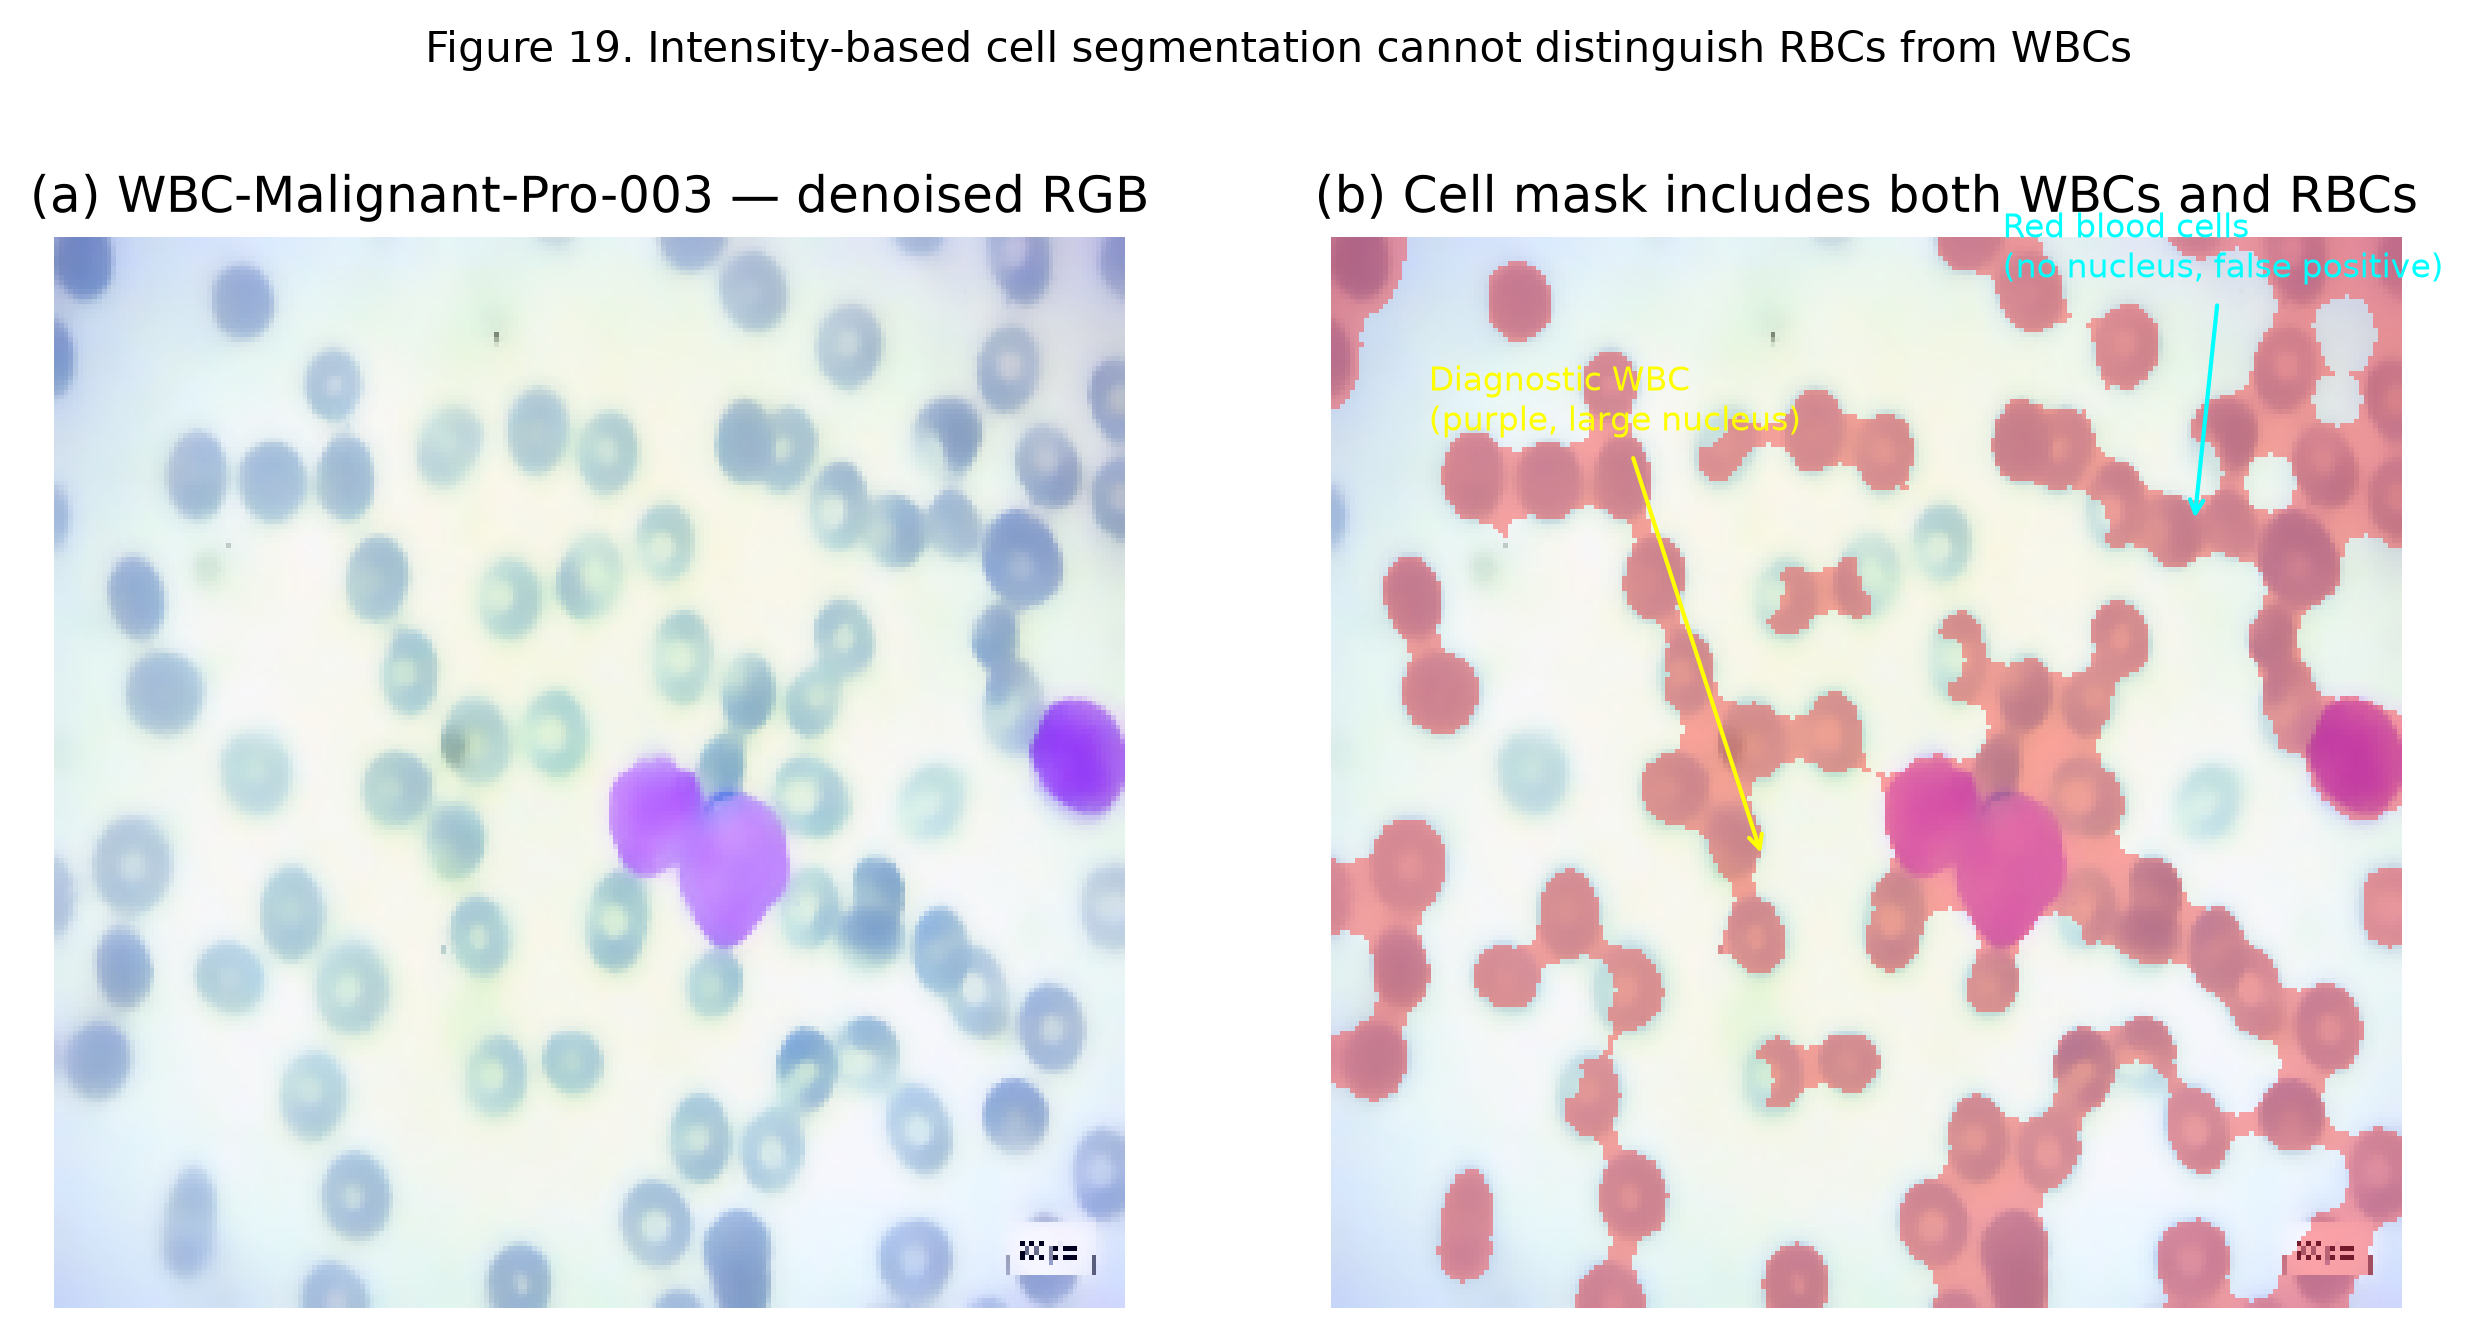
\includegraphics[width=\linewidth]{fig19_rbc_contamination.png}
  \caption{The intensity-based cell mask captures both diagnostic WBCs and non-diagnostic erythrocytes. The nucleus mask (Fig.~\ref{fig:nucseg}) already resolves this ambiguity for the downstream diagnostic signal.}
  \label{fig:rbc}
\end{figure}

\subsection{Lessons from failed methods}
The HDS analysis in Section~\ref{sec:hds} illustrates a general principle: an algorithm's applicability is constrained by the noise model it assumes. HDS is a MAP estimator under multiplicative speckle noise; applying it to additive-Gaussian-noise microscopy pushes the equations outside their region of validity, and the resulting divergence is not an implementation bug but a mathematical inevitability of the log-prior term. The two-day cost of this discovery was recovered by (i)~keeping the failing method behind a configuration switch for methodological completeness, and (ii)~documenting the analysis so that future maintainers do not repeat the experiment.

\subsection{Future work}
Extension paths in order of expected impact:
\begin{enumerate}
  \item \textbf{Watershed-based instance segmentation.} Seed watershed with the nucleus mask; use the cell mask as a foreground constraint. Yields per-cell descriptors and enables multiple-instance learning.
  \item \textbf{Colour-aware cell segmentation.} Threshold on the $a^*$ channel of $L^*a^*b^*$ (which encodes red--green opponent colour) to distinguish pink erythrocytes from purple leukocytes.
  \item \textbf{Multi-scale Hessian.} Replace APC with Frangi vesselness computed at $\sigma \in \{1.5, 2.5, 4.0\}$.
  \item \textbf{Data augmentation at training time.} 90-degree rotations, flips, and small elastic deformations to inflate the effective dataset size. WBCs are approximately rotation-invariant, making these augmentations biologically safe.
\end{enumerate}

% ==================================================================
\section{Conclusion}
\label{sec:conclusion}

We have presented a seven-stage image preprocessing pipeline for automated leukemia WBC classification, comprising stain normalization, edge-preserving denoising, three complementary feature-map computations, and a two-level intensity-based segmentation of cells and nuclei. The pipeline emits both a six-channel tensor suitable for convolutional models and a fifteen-column feature vector suitable for classical models. All intermediate results are cached to disk, decoupling preprocessing cost from training iteration cost. We have further documented and mathematically explained the divergence of the Hybrid Diffusion-Steered denoiser on natural microscopy imagery, replacing it with a bilateral filter that is both faster and correctness-preserving.

% ==================================================================
\appendices

\section{Reproducibility}
\label{app:repro}
\paragraph{Environment.} Python 3.14; NumPy 2.x; OpenCV-Python 4.x; scikit-image 0.26; SciPy 1.x; Matplotlib 3.x. All installed into a project-local virtual environment at \texttt{Manvita/.venv/}.

\paragraph{Directory layout.}
\begin{lstlisting}
Manvita/
  ml_pipeline/
    config.py            # all HPs, paths, class map
    core.py              # HDS + bilateral + APC/LOG/Canny
    stain_norm.py        # Reinhard implementation
    preprocess.py        # CLI + smoke test + main
  data/
    raw/{Benign,Early,Pre,Pro}/
    cache/{train,val,test}/*.npz
    previews/{split}/*.png
    manifest.csv
    features.csv
  docs/
    paper.tex, references.bib
    generate_figures.py
    figures/*.png
\end{lstlisting}

\paragraph{Running.}
\begin{lstlisting}
# smoke test (synthetic data)
python ml_pipeline/preprocess.py --smoke

# full run on ./data/raw
python ml_pipeline/preprocess.py

# regenerate all paper figures
python docs/generate_figures.py

# compile this paper
tectonic docs/paper.tex
\end{lstlisting}

\section{Parameter Table}
\label{app:params}
\begin{table}[h!]
  \centering
  \caption{All tunable parameters and their default values.}
  \small
  \begin{tabular}{@{}lrl@{}}
    \toprule
    Parameter & Default & Meaning \\
    \midrule
    \texttt{DENOISE\_METHOD}       & \texttt{bilateral} & \texttt{bilateral}, \texttt{hds}, or \texttt{none} \\
    \texttt{BILATERAL\_D}          & 9                 & filter neighbourhood diameter (px) \\
    \texttt{BILATERAL\_SIGMA\_COLOR}    & 75    & range Gaussian $\sigma_r$ \\
    \texttt{BILATERAL\_SIGMA\_SPACE}    & 75    & spatial Gaussian $\sigma_s$ \\
    \texttt{APC\_SIGMA}            & 2.5               & Hessian smoothing scale (px) \\
    \texttt{APC\_ALPHA}            & 0.6               & eigenvalue mixing weight \\
    \texttt{LOG\_SIGMA}            & 4.0               & LoG scale (px) \\
    \texttt{CANNY\_LOW}            & 0.10              & Canny low threshold (norm.) \\
    \texttt{CANNY\_HIGH}           & 0.25              & Canny high threshold (norm.) \\
    \texttt{NUCLEUS\_CLOSE\_RADIUS} & 3                & post-nucleus disk closing \\
    \texttt{CELL\_CLOSE\_RADIUS}   & 5                 & post-cell disk closing \\
    \texttt{MIN\_MASK\_AREA}       & 100               & minimum component size (px) \\
    \texttt{TRAIN\_RATIO}          & 0.70              & train fraction (stratified) \\
    \texttt{VAL\_RATIO}            & 0.15              & validation fraction \\
    \texttt{TEST\_RATIO}           & 0.15              & test fraction \\
    \texttt{SPLIT\_SEED}           & 42                & RNG seed for split \\
    \texttt{STAIN\_REF\_SAMPLE\_SIZE} & 20             & \# train Benign for reference \\
    \bottomrule
  \end{tabular}
\end{table}

% ==================================================================
\begin{thebibliography}{20}

\bibitem{ward2014childhood}
E.~Ward, C.~DeSantis, A.~Robbins, B.~Kohler, and A.~Jemal,
``Childhood and adolescent cancer statistics, 2014,''
\emph{CA: A Cancer Journal for Clinicians}, vol.~64, no.~2, pp.~83--103, 2014.

\bibitem{aria2021all}
M.~Aria, ``Acute Lymphoblastic Leukemia (ALL) image dataset,''
Kaggle, 2021.
\url{https://www.kaggle.com/datasets/mehradaria/leukemia}.

\bibitem{reinhard2001color}
E.~Reinhard, M.~Ashikhmin, B.~Gooch, and P.~Shirley,
``Color transfer between images,''
\emph{IEEE Computer Graphics and Applications}, vol.~21, no.~5, pp.~34--41, 2001.

\bibitem{tomasi1998bilateral}
C.~Tomasi and R.~Manduchi,
``Bilateral filtering for gray and color images,''
in \emph{Proc.\ IEEE Int.\ Conf.\ Computer Vision}, 1998, pp.~839--846.

\bibitem{frangi1998multiscale}
A.~F.~Frangi, W.~J.~Niessen, K.~L.~Vincken, and M.~A.~Viergever,
``Multiscale vessel enhancement filtering,''
in \emph{Proc.\ MICCAI}, 1998, pp.~130--137.

\bibitem{marr1980theory}
D.~Marr and E.~Hildreth,
``Theory of edge detection,''
\emph{Proc.\ Royal Soc.\ B}, vol.~207, no.~1167, pp.~187--217, 1980.

\bibitem{canny1986computational}
J.~Canny,
``A computational approach to edge detection,''
\emph{IEEE Trans.\ Pattern Anal.\ Mach.\ Intell.}, vol.~PAMI-8, no.~6, pp.~679--698, 1986.

\bibitem{haralick1973textural}
R.~M.~Haralick, K.~Shanmugam, and I.~Dinstein,
``Textural features for image classification,''
\emph{IEEE Trans.\ Systems, Man, and Cybernetics}, vol.~SMC-3, no.~6, pp.~610--621, 1973.

\bibitem{otsu1979threshold}
N.~Otsu,
``A threshold selection method from gray-level histograms,''
\emph{IEEE Trans.\ Systems, Man, and Cybernetics}, vol.~9, no.~1, pp.~62--66, 1979.

\bibitem{perona1990scale}
P.~Perona and J.~Malik,
``Scale-space and edge detection using anisotropic diffusion,''
\emph{IEEE Trans.\ Pattern Anal.\ Mach.\ Intell.}, vol.~12, no.~7, pp.~629--639, 1990.

\bibitem{opencv}
G.~Bradski, ``The OpenCV Library,''
\emph{Dr.\ Dobb's Journal of Software Tools}, 2000.

\bibitem{skimage}
S.~van~der~Walt \emph{et~al.},
``scikit-image: image processing in Python,''
\emph{PeerJ}, vol.~2, e453, 2014.

\end{thebibliography}

\end{document}
